\documentclass[a4paper,14pt]{article}
\usepackage{blindtext}
\usepackage[T2A]{fontenc}
\usepackage[utf8]{inputenc}
\usepackage[english,russian]{babel}
\usepackage{listings}
\usepackage{geometry}
\usepackage{amssymb}
\usepackage{amsmath}
\usepackage[14pt]{extsizes}
\geometry{left=2cm}
\geometry{right=1cm}
\geometry{top=2cm}
\geometry{bottom=2cm}
\pagestyle{plain}
\usepackage{pgfplots}
\usepackage{filecontents}
\usepackage{graphicx}
\usepackage{indentfirst}
\DeclareGraphicsExtensions{.png}
\graphicspath{{images/}}
\usetikzlibrary{datavisualization}
\usetikzlibrary{datavisualization.formats.functions}
\usepackage{tabularx}
\pgfplotsset{width=7 cm}
\usepackage{xcolor}
%\renewcommand{\rmdefault}{ftm}
%\usepackage{mathptmx}
\usepackage{setspace}
%\полуторный интервал
\onehalfspacing
\frenchspacing

\usepackage{tocloft}

\renewcommand{\cftsecdotsep}{\cftdot}
\renewcommand{\cftsecleader}{\cftdotfill{\cftsecdotsep}}
\renewcommand{\cftsubsecleader}{\cftdotfill{\cftsecdotsep}}
\renewcommand{\cftsubsubsecleader}{\cftdotfill{\cftsecdotsep}}

%\renewcommand\cftchapdotsep{\cftdot}
%\renewcommand\cftsecdotsep{\cftdot}
%\renewcommand{\cftchapleader}{\cftdotfill{\cftchapdotsep}}

% Для измененных титулов глав:
% % подключаем нужные пакеты
%\definecolor{gray75}{gray}{0.75} % определяем цвет
%\newcommand{\hsp}{\hspace{20pt}} % длина линии в 20pt
% titleformat определяет стиль
%\titleformat{\chapter}[hang]{\Huge\bfseries}{\thechapter\hsp\textcolor{black}{|}\hsp}{0pt}{\Huge\bfseries}
%\usepackage{titlesec, blindtext, color}
%\titleformat{\chapter}[hang]{\Huge\bfseries}{\thechapter\hsp\textcolor{black}{|}\hsp}{0pt}{\Huge\bfseries}

% Для листинга кода:
\lstset{ %
language=python,                 % выбор языка для подсветки
basicstyle=\small\sffamily, % размер и начертание шрифта для подсветки кода
numbers=left,               % где поставить нумерацию строк (слева\справа)
numberstyle=\tiny,           % размер шрифта для номеров строк
stepnumber=1,                   % размер шага между двумя номерами строк
numbersep=5pt,                % как далеко отстоят номера строк от подсвечиваемого кода
showspaces=false,            % показывать или нет пробелы специальными отступами
showstringspaces=false,      % показывать или нет пробелы в строках
showtabs=false,             % показывать или нет табуляцию в строках
frame=single,              % рисовать рамку вокруг кода
tabsize=4,                 % размер табуляции по умолчанию равен 2 пробелам
captionpos=t,              % позиция заголовка вверху [t] или внизу [b]
breaklines=true,           % автоматически переносить строки (да\нет)
breakatwhitespace=false, % переносить строки только если есть пробел
escapeinside={\#*}{*)},   % если нужно добавить комментарии в коде
literate={а}{{\selectfont\char224}}1
{б}{{\selectfont\char225}}1
{в}{{\selectfont\char226}}1
{г}{{\selectfont\char227}}1
{д}{{\selectfont\char228}}1
{е}{{\selectfont\char229}}1
{ё}{{\"e}}1
{ж}{{\selectfont\char230}}1
{з}{{\selectfont\char231}}1
{и}{{\selectfont\char232}}1
{й}{{\selectfont\char233}}1
{к}{{\selectfont\char234}}1
{л}{{\selectfont\char235}}1
{м}{{\selectfont\char236}}1
{н}{{\selectfont\char237}}1
{о}{{\selectfont\char238}}1
{п}{{\selectfont\char239}}1
{р}{{\selectfont\char240}}1
{с}{{\selectfont\char241}}1
{т}{{\selectfont\char242}}1
{у}{{\selectfont\char243}}1
{ф}{{\selectfont\char244}}1
{х}{{\selectfont\char245}}1
{ц}{{\selectfont\char246}}1
{ч}{{\selectfont\char247}}1
{ш}{{\selectfont\char248}}1
{щ}{{\selectfont\char249}}1
{ъ}{{\selectfont\char250}}1
{ы}{{\selectfont\char251}}1
{ь}{{\selectfont\char252}}1
{э}{{\selectfont\char253}}1
{ю}{{\selectfont\char254}}1
{я}{{\selectfont\char255}}1
{А}{{\selectfont\char192}}1
{Б}{{\selectfont\char193}}1
{В}{{\selectfont\char194}}1
{Г}{{\selectfont\char195}}1
{Д}{{\selectfont\char196}}1
{Е}{{\selectfont\char197}}1
{Ё}{{\"E}}1
{Ж}{{\selectfont\char198}}1
{З}{{\selectfont\char199}}1
{И}{{\selectfont\char200}}1
{Й}{{\selectfont\char201}}1
{К}{{\selectfont\char202}}1
{Л}{{\selectfont\char203}}1
{М}{{\selectfont\char204}}1
{Н}{{\selectfont\char205}}1
{О}{{\selectfont\char206}}1
{П}{{\selectfont\char207}}1
{Р}{{\selectfont\char208}}1
{С}{{\selectfont\char209}}1
{Т}{{\selectfont\char210}}1
{У}{{\selectfont\char211}}1
{Ф}{{\selectfont\char212}}1
{Х}{{\selectfont\char213}}1
{Ц}{{\selectfont\char214}}1
{Ч}{{\selectfont\char215}}1
{Ш}{{\selectfont\char216}}1
{Щ}{{\selectfont\char217}}1
{Ъ}{{\selectfont\char218}}1
{Ы}{{\selectfont\char219}}1
{Ь}{{\selectfont\char220}}1
{Э}{{\selectfont\char221}}1
{Ю}{{\selectfont\char222}}1
{Я}{{\selectfont\char223}}1
}

\begin{document}
\setcounter{page}{2}
\tableofcontents

\newpage
\section*{Введение}
\addcontentsline{toc}{section}{Введение}

Иногда при работе с Linux-системами необходимо осуществлять перехват вызовов функций внутри ядра (например, открытие файлов или каталогов) для обеспечения возможности мониторинга активности в системе или превентивного блоки­рования деятельности подозрительных процессов.
Перехват вызовов функций внутри ядра может осуществляться различными способами, такими как использование LSM, модификация таблицы системных вызовов, использование kpro-bes, использование cплайсинга и использование ftrace.

В настоящее время в официальное ядро Linux входят, например, такие security-модули, как AppArmor, SELinux, Smack и TOMOYO. Кроме того, с версии Linux 2.6.1 введена поддержка systrace. Systrace -- это служебная программа для обеспечения компьютерной безопасности, которая ограничивает доступ приложений к системе, применяя политики доступа для системных вызовов. Systrace особенно полезен при запуске ненадежных приложений.

Данная работа посвящена исследованию способов перехвата системных вызовов. Целью проекта является разработка загружаемого модуля ядра, позволяющего перехватывать системные вызовы для отслеживания событий файловой системы.


\newpage
\section{Аналитический раздел}

В соответствии с заданием на курсовой проект необходимо разработать загружаемый модуль ядра, перехватывающий системные вызовы, связанные с событиями в файловой системе Linux. Модуль должен осуществлять наблюдение за всеми файлами и директориями, записанными в конфигурационный файл модуля. Модуль должен отслеживать следущие события (в скобках указаны соответсвтующие системные вызовы):

\begin{itemize}
	\item открытие файла (openat());
	\item создание файла (creat());
	\item запись данных в открытый файл (write()); 
	\item удаление записи из файла каталога (unlink(), unlinkat());
	\item создание каталога (mkdir(), mkdirat()).
\end{itemize}

Все произошедшие события модуль должен записывать в log-файл для того, чтобы впоследствии эту информацию можно было считать из пространства пользователя.

Для понимания алгоритма перехвата системных вызовов необходимо сначала рассмотреть, как происходит системный вызов.

\subsection{Траектория системного вызова}

Системный вызов - это фундаментальный интерфейс между приложением уровня пользователя и ядром Linux. Большую часть времени программы выполняются в пользовательском режиме и переключаются в режим ядра только тогда, когда им требуется служба операционной системы. Услуги операционной системы предоставляются через системные вызовы. Системные вызовы -- это «ворота» в ядро, реализованные с помощью программных прерываний. Программные прерывания -- это прерывания, создаваемые программой и обрабатываемые операционной системой в режиме ядра. Операционная система поддерживает «таблицу системных вызовов», в которой есть указатели на функции, реализующие системные вызовы внутри ядра.

В любой (в том числе и микроядерной) операционной системе системный вызов выполняется некоторой выделенной процессорной инструкцией, прерывающей последовательное выполнение команд и передающий управление коду режима супервизора. Это обычно некая команда программного прерывания, в зависимости от архитектуры процессора в разные времена это были команды с мнемониками вида: svc, emt, trap, int и им подобными. Если обратиться только к архитектуре Intel x86, то в ней для этого традиционно используется команда программного прерывания с различным вектором. Начиная с определенного момента (примерно с начала 2008 года или момента выхода Windows XP Service Pack 2) многие операционные системы (Windows, Linux) отказались от использования программного прерывания int, и перешли к реализации системного вызова и возврата из него через новые команды процессора sysenter (sysexit) \cite{zirulnik}, однако ничего принципиально нового не появилось.

Системные вызовы обычно вызываются не напрямую, а через функции оболочки в glibc (или, возможно, в какой-либо другой библиотеке). Все системные вызовы далее преобразуются в вызов ядра функцией syscall(), 1-м параметром которого будет идентификатор выполняемого системного вызова, например \_\_NR\_execve.

Системный вызов syscall(), попав в ядро, всегда попадает в таблицу sys\_call\_table, и далее переадресовывается по индексу (смещению) в этой таблице на величину 1-го параметра вызова syscall() - идентификатора требуемого системного вызова \cite{zirulnik}.

Рассмотрим теперь возможные способы перехвата системных вызовов в Linux.

\subsection{Анализ подходов реализации перехвата системных вызовов}

Сущетсвуют следующие способы реализации перехвата системных вызовов в Linux:

\begin{itemize}
	\item Linux Security Modules (LSM);
	\item модификация таблицы системных вызовов;
	\item использование kprobes;
	\item cплайсинг;
	\item использование ftrace.
\end{itemize}

\subsubsection{Linux Security Modules}

Интерфейс LSM позволяет ядру Linux поддерживать различные модели компьютерной безопасности. LSM был создан для решения проблемы контроля доступа и является частью ядра начиная с Linux версии 2.6. LSM вставляет перехватчики (security-функций, которые в свою очередь вызывают обратные вызовы, установленные security-модулем) в каждую критическую точку ядерного кода, где системные вызовы уровня пользователя получают доступ к важным внутренним объектам ядра, таким как inode. Security-модуль может изучать контекст операции и принимать решение о её разрешении или запрете.

В частности, для файловых операций были определены три набора перехватчиков: перехватчики файловой системы, перехватчики inode и перехватчики файлов. LSM добавляет поле безопасности в каждую из связанных структур данных ядра: суперблок, индексный дескриптор и файл. Перехватчики файловой системы позволяют модулям безопасности управлять такими операциями, как, например, монтирование.

Название «модуль» несколько неверно, поскольку security-модули на самом деле не являются загружаемыми модулями ядра, а подключаются к ядру во время его сборки. Соответственно, Linux Security API имеет важное ограничение: security-модули не могут быть загружены динамически, являются частью ядра и требуют его пересборки. 

Таким образом, несмотря на то, что LSM был разработан именно для мониторинга системных вызовов, для его использования необходимо поставлять собственную сборку ядра, а также интегрировать дополнительный модуль с SELinux или AppArmor, которые используются популярными дистрибутивами.

\subsubsection{Модификация таблицы системных вызовов}

Cохранив старое значения обработчика и подставив в таблицу системных собственный обработчик, мы можем перехватить любой системный вызов. Таблица указателей на функции ядра, которые реализуют системные вызовы, расположена в
массиве sys\_call\_table. Такой подход известен программистам еще со времен MS-DOS.

Для перехвата системных этим способом используется механизм загружаемых модулей ядра. Для реализации модуля, перехватывающего системный вызов, необходимо определить алгоритм перехвата. Алгоритм следующий:

\begin{enumerate}
	\item сохранить указатель на оригинальный (исходный) вызов для возможности его восстановления;
	\item создать функцию, реализующую новый системный вызов;
	\item в таблице системных вызовов sys\_call\_table произвести замену вызовов, т.е настроить соответствующий указатель на новый системный вызов;
	\item по окончании работы (при выгрузке модуля) восстановить оригинальный
	системный вызов, используя ранее сохраненный указатель.
\end{enumerate}

Данный подход имеет следующие преимущества:

\begin{itemize}
	\item полный контроль над любыми системными вызовами;
	\item минимальные накладные расходы;
	\item минимальные требования к ядру.
\end{itemize}

Однако метод имеет и недостатки:

\begin{itemize}
	\item техническая сложность реализации (необходимо найти таблицу системных вызовов, обойти защиту от модификации таблицы, выполнить замену атомарно и безопасно);
	\item невозможность перехвата некоторых обработчиков (некоторые обработчики реализованы на языке ассемблера, и их сложно или даже невозможно заменить на свои обработчики, написанные на C);
	\item перехватываются только системные вызовы (точки входа ограничиваются только системными вызовами, а все дополнительные проверки выполняются либо до непосредственного сиситемного вызова, либо после, поэтому необходимо дублировать проверки на адекватность аргументов).
\end{itemize}

\subsubsection{Использование kprobes}

Kprobes -- это механизм отладки для ядра Linux, который также можно использовать для мониторинга событий внутри ядра. Этот механизм позволяет вставлять точки останова в работающее ядро.
С помощью kprobes можно прервать выполнение ядерного кода в любом месте и вызвать свой обработчик.
Этот интерфейс позволяет устанавливать пред- и постобработчики для любой инструкции в ядре, а также обработчики на вход и возврат из функции.

Для добавления своего собственного зонда (probe) в работающее ядро необходимо написать загружаемый модуль ядра, который реализует предварительный обработчик и пост-обработчик для зондирования.

Преимущества использования kprobes:

\begin{itemize}
	\item зрелый API. Kprobes существуют и улучшаются с 2002 года;
	\item перехват любого места в ядре. Kprobes реализуются с помощью точек оста­нова (инструкции int3), внедряемых в исполнимый код ядра. Это позволяет устанав­ливать kprobes в буквально любом месте любой функции, если оно известно.
\end{itemize}

Недостатки kprobes:

\begin{itemize}
	\item техническая сложность. Kprobes — это только способ установить точку оста­нова в любом места ядра. Для получения аргументов функции или значений ло­кальных переменных надо знать, в каких регистрах или где на стеке они лежат, и самостоятельно их оттуда извлекать;
	\item ограничения kretprobes. Kretprobes реализуются через подмену адреса возврата на стеке. Соответственно, им необходимо где-то хранить оригинальный адрес, чтобы вернуться туда после обработки kretprobe. Адреса хранятся в буфере фиксированного размера. В случае его переполнения, когда в системе выполняется слишком много одновременных вызовов перехваченной функции, kretprobes будет пропускать срабатывания;
	\item при обработке зондов (probes) приоритетное прерывание отключено. Это накладывает определённые ограничения на обработчики: в них нельзя выполнять операции ввода-вывода, спать в таймерах и семафорах;
	\item В текущей реализации kprobes существуют некоторые задержки в работе, причиной которых является kprobe\_lock, который сериализует выполнение зондов на всех ЦП на машине SMP. Другая причина -- это механизм kprobes, который использует несколько исключений для обработки одного зонда. Обработка исключений -- дорогостоящая операция, которая вызывает задержки. 
\end{itemize}

\subsubsection{Сплайсинг}

Сплайсинг -- это метод перехвата функций путём изменения кода целевой функции. Инструкции в начале целевой функциии заменяются на безусловный переход, ведущий в нужный нам обработчик. Оригинальные инструкции переносятся в другое место и исполняются перед переходом обратно в перехваченную функцию. С помощью двух переходов мы вшиваем (splice in) свой дополнительный код в функцию, поэтому такой подход называется сплайсингом. Методом сплайсинга реализована jump-оптимизация для kprobes.

Преимущества сплайсинга:

\begin{itemize}
	\item минимальные требования к ядру. Сплайсинг не требует каких-либо особенных опций в ядре и работает в начале любой функции. Нужно только знать её адрес;
	\item минимальные накладные расходы. Необходимо всего лишь два безусловных перехода. Подобные переходы отлично предсказываются процессором и являются очень дешёвыми.
\end{itemize}

Однако сплайсинг имеет один серьезный недостаток: высокая техническая сложность реализации. Нельзя просто так взять и переписать машинный код. Для этого необходимо синхронизировать установку и снятие перехвата; обойти защиту на модификацию регионов памяти с кодом; дизассемблировать заменяемые инструкций, чтобы скопировать их целыми. В режиме ядра необходимо запретить прерывания для избежания переключения задач, так как при замене кода в начале функции перехватываемая функция может понадобиться другому потоку.

\subsubsection{Использование ftrace}

Ftrace — это внутренний трассировщик ядра, позволяющий разработчикам посмотреть, что происходит внутри ядра системы. Ftrace был включен в основную линию ядра Linux в версии 2.6.27, выпущенной в 2008 году. С помощью ftrace можно отслеживать контекстные переключения, измерять время обработки прерываний, высчитывать время на активизацию заданий с высоким приоритетом и многое другое.

Ftrace полагается на механизм профилирования gcc для добавления машинных инструкций к скомпилированным версиям всех функций ядра, которые перенаправляют выполнение функций на плагины трассировщика ftrace, которые выполняют фактическую трассировку. В начало каждой функции добавляется вызов специальной трассировочной функции mcount() или \_\_fentry\_\_(). 

Ftrace поддерживает динамическое отслеживание вызовов функций ядра. Ядро знает расположение всех вызовов mcount() или \_\_fentry\_\_() и на ранних этапах загрузки заменяет их машинный код на nop — специальную инструкцию, которая предписывает ничего не делать. При включении трассирования в нужные функции вызовы ftrace добавляются обратно. Таким образом, если ftrace не используется, то его влияние на систему минимально.

Преимущества использования данного подхода: 

\begin{itemize}
	\item зрелый API и простой код. Использование готовых интерфейсов в ядре су­щественно упрощает код. Вся установка перехвата требует пары вызовов функций,заполнение двух полей в структуре;
	\item подход автоматически совместим с вытеснением, в отличие от kprobes;
	\item нет ограничений на функции. Подход с ftrace лишён недостатка kretprobes и из коробки поддерживает любое количество активаций перехватываемой функции;
	\item перехват любой функции по имени. Можно перехватить любую функцию (даже неэкспортируемую для модулей), зная лишь её имя;
	\item перехват совместим с трассировкой. Очевидно, что этот способ не конфлик­тует с ftrace, так что с ядра всё ещё можно снимать очень полезные показатели производительности.
\end{itemize}

\newpage
Однако, ftrace, как и другие подходы, не лишен недостатков:

\begin{itemize}
	\item требования к конфигурации ядра. Для поддержки ftrace ядро должно предоставлять целый ряд возможностей (список символов kallsyms для поиска функций по имени; фреймворк ftrace в целом для выполнения трассировки; опции ftrace, критически важные для перехвата
	);
	\item оборачиваются целиком вызовы функций. ftrace срабатывает исключительно при входе;
\end{itemize}

Несмотря на описанные недостатки следует учитывать, что обычно ядра, используемые популярными дистрибутивами, все необходимые ftrace опции в себе всё равно содержат, так как они не влияют на производительность и полезны при отладке. Иметь в виду эти требования стоит, если необходимо поддерживать какие-то особенные ядра. Оборачивание функций целиком в целом удобно, но для каких-либо специфических задач может и не подходить.

При использовании ftrace стоит учитывать, что использование kprobes или сплайсинга может помешать меха­низмам ftrace.

%\subsection{Вывод}
%\addcontentsline{toc}{section}{Вывод}

%В данном разделе были проанализированы возможные подходы к реализации перехвата системных вызовов.

%Для использования LSM необходима пересборка ядра и интеграция нового модуля с AppArmor, SELinux, Smack и TOMOYO, которые используются в популярных дистрибутивах. Модификация таблицы системных вызовов, использование kprobes или сплайсинга характеризуются высокой технической сложностью реализации. Поэтому наиболее подходящим вариантом является использование трассировщика ftrace.

\newpage
\section{Конструкторский раздел}

В данном разделе

\subsection{Общая архитектура приложения}

Для реализации подхода с ftrace необходимо реализовать загружаемый модуль ядра. В состав разрабатываемого программного обеспечения входит только загружаемый модуль ядра, следящий за необходимыми системными вызовами с последующим выводом информации в лог-файл.

\subsection{Перехват системных вызовов}

Перехватываемую функцию можно описать следующей структурой (листинг \ref{lst:ftrace_hook}).


\begin{lstlisting}[language=C++,label={lst:ftrace_hook}, caption=\text{ftrace\_hook.}]
/**
* struct ftrace_hook - описывает перехватываемую функцию
*
* @name:       имя перехватываемой функции
*
* @function:   адрес функции-обёртки, которая будет вызываться вместо
*              перехваченной функции
*
* @original:   указатель на место, куда следует записать адрес
*              перехватываемой функции, заполняется при установке
*
* @address:    адрес перехватываемой функции, выясняется при установке
*
* @ops:        служебная информация ftrace, инициализируется нулями,
*              при установке перехвата будет доинициализирована
*/
struct ftrace_hook
{
   const char *name;
   void *function;
   void *original;
   
   unsigned long address;
   struct ftrace_ops ops;
};   
\end{lstlisting}

Пользователю необходимо заполнить только первые три поля: name, function, original. Остальные поля считаются деталью реализации. Описание всех перехватываемых функций можно собрать в массив и использовать макросы, чтобы повысить компактность кода (листинг\ref{lst:hooks}).

\begin{lstlisting}[language=C++,label={lst:hooks}, caption=\text{Описание перехватываемых функций.}]
#define HOOK(_name, _function, _original)       \
{                                       \
	.name = (_name),                    \
	.function = (_function),            \
	.original = (_original),            \
}

static struct ftrace_hook fs_hooks[] = {
	HOOK("sys_mkdir", fh_sys_mkdir, &real_sys_mkdir),
	HOOK("sys_openat", fh_sys_openat, &real_sys_openat),
	HOOK("sys_creat", fh_sys_creat, &real_sys_creat),
	HOOK("sys_unlink", fh_sys_unlink, &real_sys_unlink),
	HOOK("sys_write", fh_sys_write, &real_sys_write),
	HOOK("sys_unlinkat", fh_sys_unlinkat, &real_sys_unlinkat),
	HOOK("sys_mkdirat", fh_sys_mkdirat, &real_sys_mkdirat)
};	
\end{lstlisting}

Обёртки над перехватываемыми функциями выглядят следующим образом (листинг \ref{lst:wraps}).

\begin{lstlisting}[language=C++,label={lst:wraps}, caption=\text{Обёртки над перехватываемыми функциями .}]
// настоящий обработчик системного вызова mkdir
static asmlinkage long (*real_sys_mkdir)(struct pt_regs *regs);

// наш обработчик системного вызова mkdir
static asmlinkage long fh_sys_mkdir(struct pt_regs *regs)
{
	long ret;

	ret = real_sys_mkdir(regs);

	// ...
	returnt ret;
}
\end{lstlisting}

Важно, чтобы сигнатуры функций в точности совпадали. Без этого, очевидно, аргументы будут переданы неправильно и всё пойдёт под откос.

\subsection{Открытие, чтение из файлов и запись в файлы из пространства ядра}

Открытие файлов в ядре производится с помощью функции filp\_open(). Эта функция возвращает указатель на структуру struct file -- структуру, описывающую открытый процессом файл (листинг \ref{lst:sfile}).

\begin{lstlisting}[language=C++,label={lst:sfile}, caption=\text{struct file для ядра версии 5.4.}]
struct file {
	union {
		struct llist_node	fu_llist;
	struct rcu_head 	fu_rcuhead;
	} f_u;
	struct path		f_path;
	struct inode		*f_inode;	/* cached value */
	const struct file_operations	*f_op;
	//...
	unsigned int 		f_flags;
	fmode_t			f_mode;
	struct mutex		f_pos_lock;
	loff_t			f_pos;
	// ...
};
\end{lstlisting}

Структура struct file, в частности, содержит указатель на inode файла (struct inode *), которая содержит поле umode\_t i\_mode. Это поле можно передать макросу S\_ISDIR(), определенному в <<linux/stat.h>>. Макрос S\_ISDIR() определит, является файл директорией или нет.

Чтение из файла выполняется с помощью функции kernel\_read(), а запись -- с помощью функции kernel\_write(). Сигнатуры функций filp\_open(),  kernel\_read() и kernel\_write() приведены в листинге \ref{lst:signats}.

\newpage
\begin{lstlisting}[language=C++,label={lst:signats}, caption=\text{filp\_open(),  kernel\_read() и kernel\_write() для ядра версии 5.4.}]
struct file *filp_open(const char *, int, umode_t);

ssize_t kernel_read(struct file *, void *, size_t, loff_t *);

ssize_t kernel_write(struct file *, const void *, size_t, loff_t *);
\end{lstlisting}

\subsection{Поиск имен файлов, открытых процессом, по номеру файлового дескриптора}

В разрабатываемом модуле ядра необходимо осуществлять мониторинг за файлами и директориями. В конфигурационном файле модуля записаны имена файлов и директорий, однако в системные вызовы могут передаваться не только абсолютные пути до файлов, но и относительные, а, например, в системный вызов write передается только номер дескриптора открытого файла. То есть необходимо осуществить поиск имени файла, зная номер его файлового дескриптора и PID открывшего его процесса. Помочь с этим может виртуальная файловая система /proc.

Файловая система /proc содержит каталоги (для структурирования информации) и виртуальные файлы. Виртуальный файл, как уже было сказано, может предоставлять пользователю информацию, полученную из ядра и, кроме того, служить средством передачи в ядро пользовательской информации. /proc, в частности, содержит каталоги, содержащие информацию о выполняющихся в системе процессах. Каждому запущенному процессу соответствует подкаталог с именем, соответствующим идентификатору этого процесса (его pid). (/proc/<PID>). Каждый из этих каталогов содержит, кроме всего прочего, подкаталог fd, содержащий одну запись на каждый файл, который в данный момент открыт процессом. Имя каждой такой записи соответствует номеру файлового дескриптора и является символьной ссылкой на реальный файл (/proc/<PID>/fd/N).

Чтобы получить информацию об имени файла, используя /proc/<PID>/fd/N, необходимо выполнить следующие шаги.

\begin{enumerate}
	\item Открыть файл /proc/<PID>/fd/N для чтения с помощью функции filp\_open().
	\item Получить поле f\_path, являющейся структурой struct path из указателя на структуру struct file, который вернула функция filp\_open().
	\item Вызвать функцию path\_get и передать ей указатель на полученную на предыдущем шаге структуру struct path. Ее сигнатура приведена в листинге \ref{lst:d_path}.
	\item Вызвать функцию d\_path, ее сигнатура приведена в листинге \ref{lst:d_path}. Она вернет абсолютный путь до необходимого файла. 
\end{enumerate}

\begin{lstlisting}[language=C++,label={lst:d_path}, caption=\text{d\_path() и path\_get() для ядра версии 5.4.}]
char *d_path(const struct path *, char *, int);

void path_get(const struct path *);
\end{lstlisting}


\subsection{Адреса функций и процедур ядра}

Виртуальная файловая система /proc содержит псевдофайл /proc/kallsyms -- файл, внутри которого находится символьная таблица адресов функций и процедур, используемых ядром операционной системы Linux. В этой таблице перечислены имена переменных и функций и их адреса в памяти компьютера. В отличие от System.map, /proc/kallsyms содержит таблицу символов не только статически, но и динамически загружаемых модулей.

Псевдофайл /proc/kallsyms (таблица) - это ни что иное, как отображение во внешнее окружение некоторой внутренней структуры ядра. Ядро предоставляет пользователям (т.е. модулям) вызов kallsyms\_lookup\_name(), позволяющий выполнять поиск в этой внутренней структуре.

Однако kallsyms\_lookup\_name() присутствует в версиях ядра, начиная 2.6.32. Кроме того, начиная с версии 5.6, этот символ не экспортируется, поэтому неоюходим другой механизм поиска по /proc/kallsyms. В данной работе используется ядро версии 5.4, где этот символ является экспортируемым.

\subsection{Алгоритм работы перехвата с импользованием ftrace}

Рассмотрим следующий пример. При наборе в терминале команды ls, командный интерпретатор (Bash) для запуска нового процесса использует функции функций fork() + execve(). Внутри эти функции реализуются через системные вызовы clone() и execve() соответственно. Допустим, мы перехватываем системный вызов execve(), чтобы контролировать запуск новых процессов.

В графическом виде перехват функции-обработчика выглядит так, как показано на рисунке \ref{fig:lshook}.

\begin{figure}[!h]
    \center{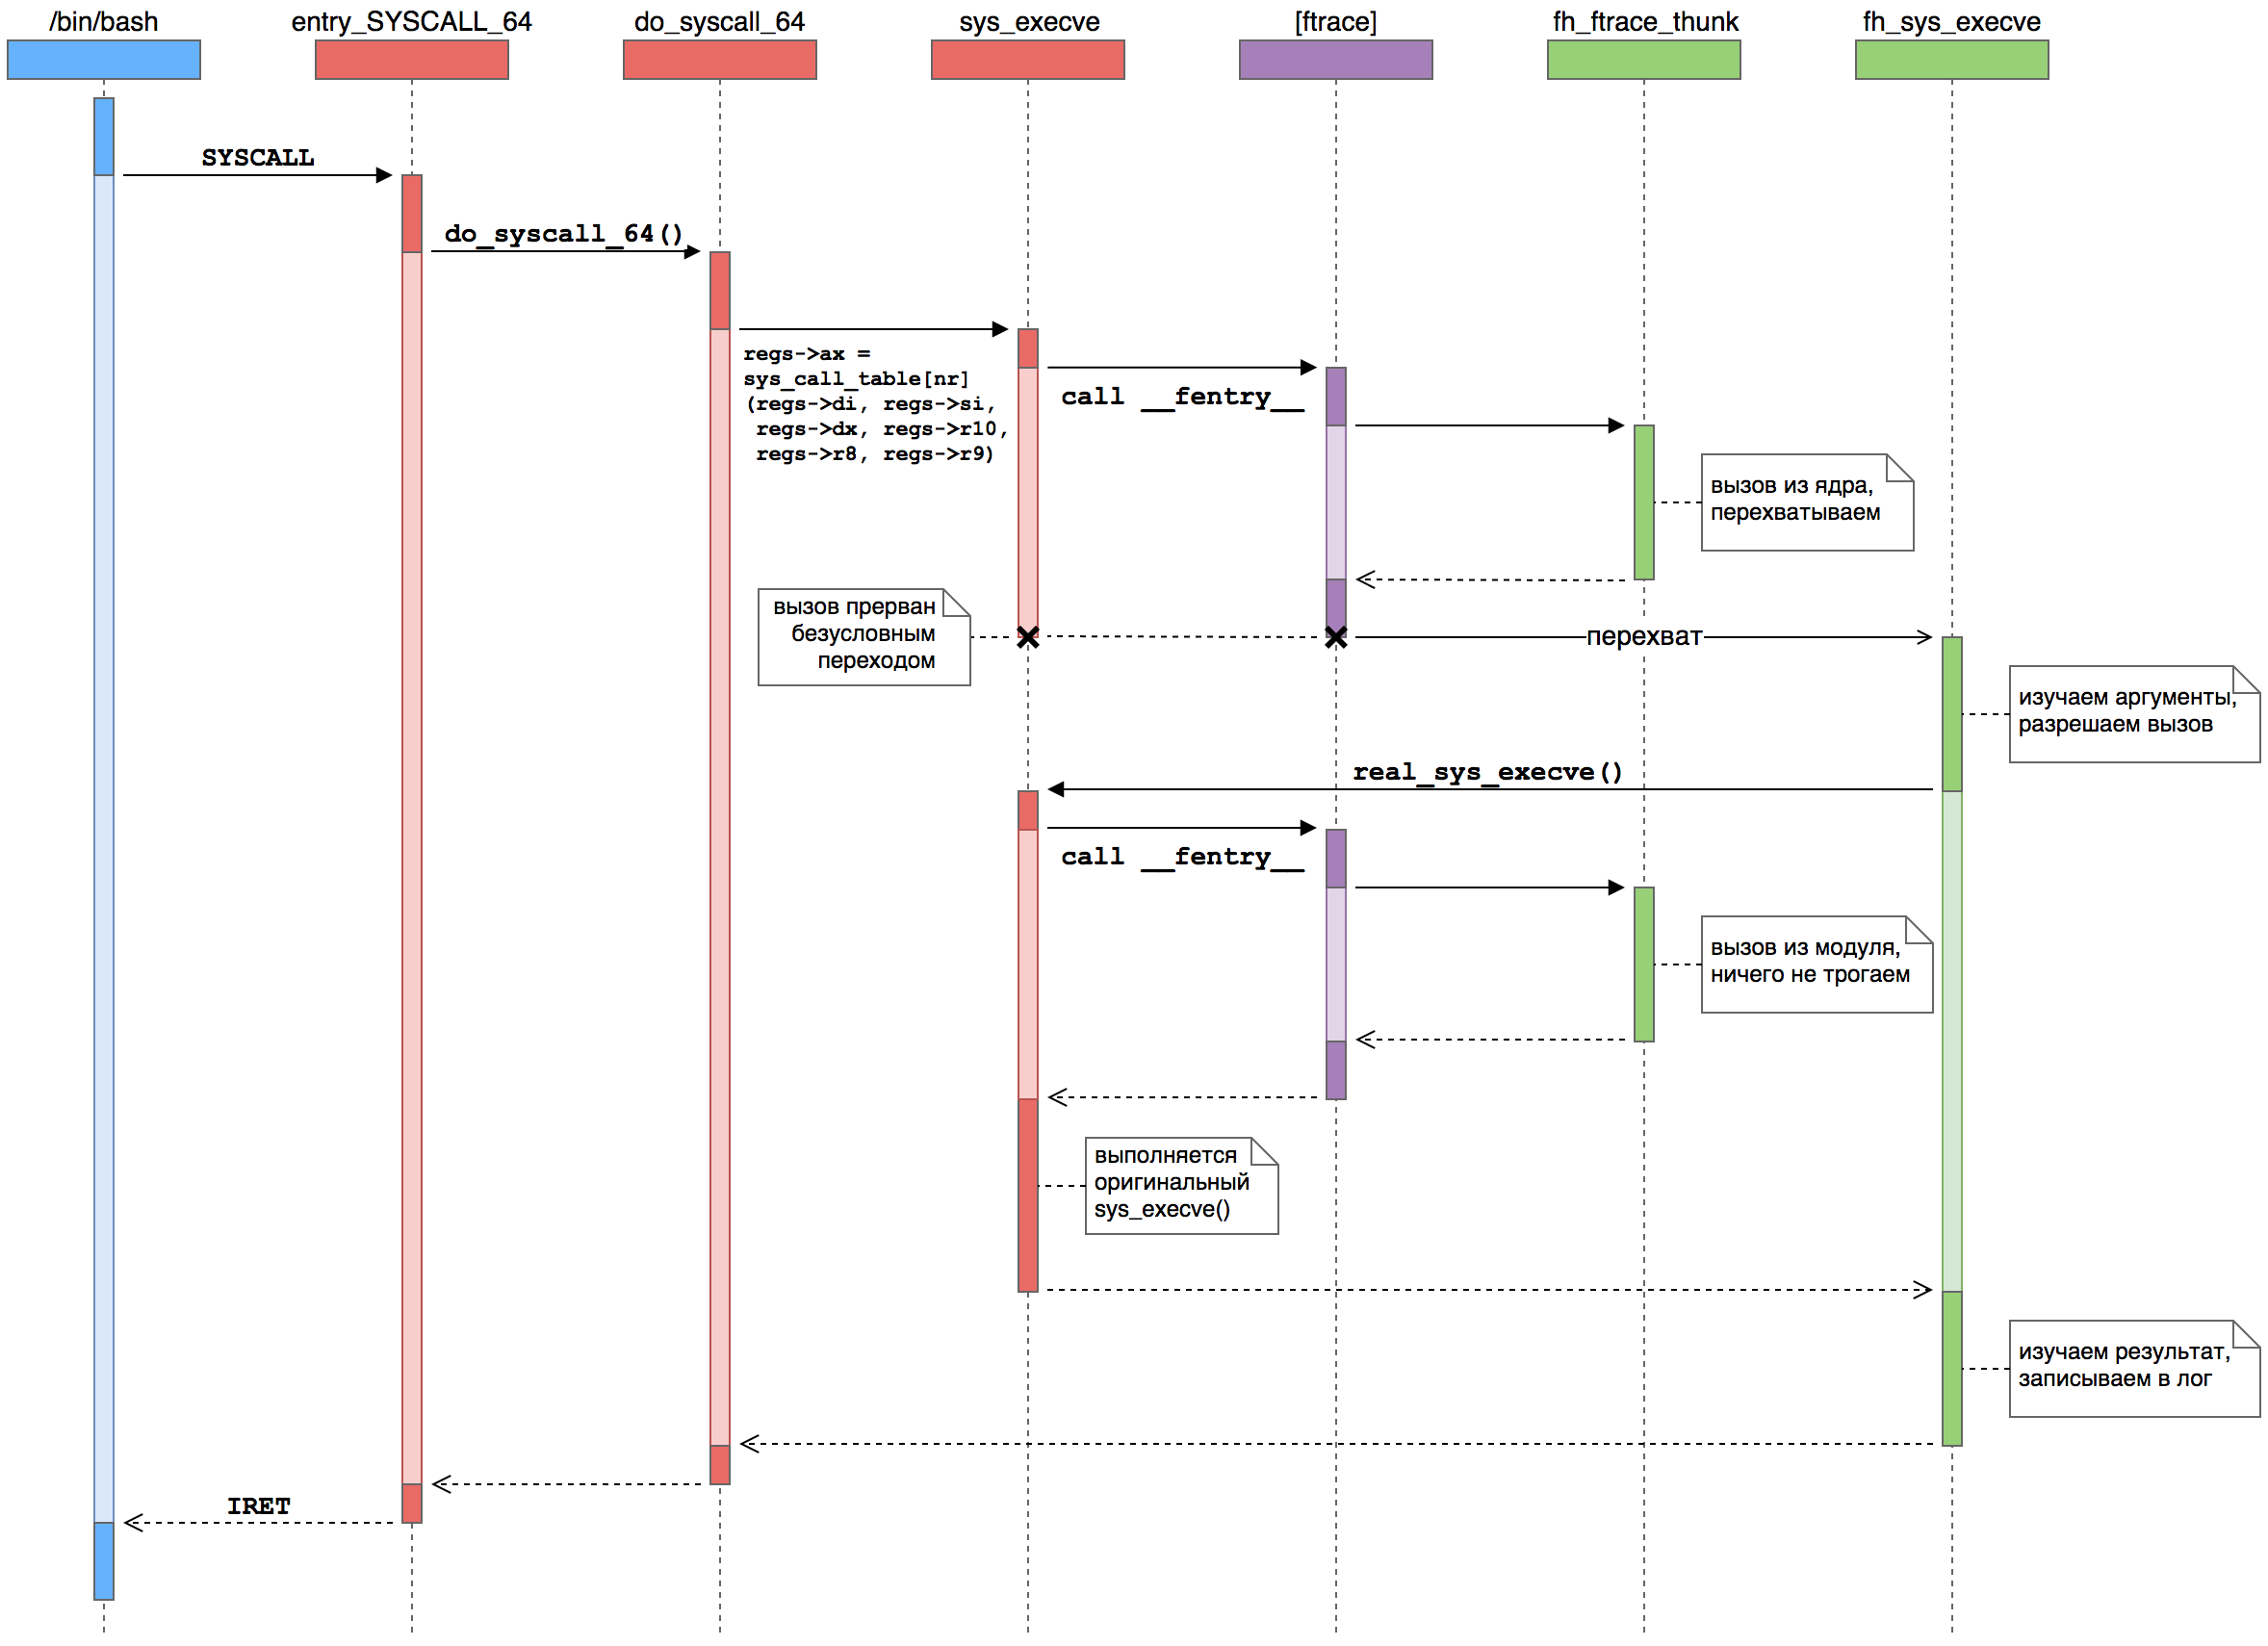
\includegraphics[width=16cm]{img/lshook}}
    \caption{Схема перехвата системного вызова execve() \cite{ftrace}.}
    \label{fig:lshook}
\end{figure}

Пользовательский процесс (отмечен голубым) выполняет системный вызов в ядро (красный), где ftrace (фиолетовый) выполняет безусловный переход в функцию из нашего модуля (зеленый). Можно выделить следующие шаги при выполнении перехвата системного вызова на 64-битных ядрах.

\begin{enumerate}
	\item Пользовательский процесс выполняет SYSCALL. С помощью этой инструкции выполняется переход в режим ядра и управление передаётся низкоуровневому обработчику системных вызовов — entry\_SYSCALL\_64(). Он отвечает за все системные вызовы 64-битных программ на 64-битных ядрах.
	\item Управление переходит к конкретному обработчику. Вызывается функция do\_syscall\_64(), которая в свою очередь обращается к таблице обработчиков системных вызовов sys\_call\_table и вызывает оттуда конкретный обработчик по номеру системного вызова.
	\item Вызывается ftrace. В начале каждой функции ядра находится вызов функции \_\_fentry\_\_(), которая реализуется фреймворком ftrace.
	\item Ftrace вызывает наш коллбек. В процессе работы ftrace вызывает все зарегистрированные трассировочные коллбеки, включая и наш.
	\item Коллбек из нашего модуля принимает решение о выполнении перехвата (если он обнаружит рекурсию, то перехват не будет выполнен, иначе произойдет зависание системы).
	\item Ftrace восстанавливает регистры. Ftrace сохраняет состояние регистров в структуре pt\_regs перед вызовом обработчиков. При завершении обработки ftrace восстанавливает регистры из этой структуры. Наш обработчик изменяет регистр \%rip — что в итоге приводит к передаче управления по новому адресу.
	\item Управление получает функция-обёртка из нашего модуля. При этом всё остальное состояние процессора и памяти остаётся без изменений, поэтому наша функция получает все аргументы оригинального обработчика и при завершении вернёт управление в функцию do\_syscall\_64().
	\item Обёртка вызывает оригинальную функцию. Наша функция-обертка может проанализировать аргументы и контекст системного вызова (кто что запускает) и, например, запретить или разрешить процессу его выполнение. В случае запрета функция просто возвращает код ошибки. Иначе через указатель real\_sys\_execve, который был сохранён при настройке перехвата, вызывается оригинальный обработчик.
	\item Управление получает коллбек. Как и при первом вызове, управление опять проходит через ftrace и передаётся в наш коллбек. Однако в этот раз он ничего не делает, потому что в этот раз вызов просиходит из нашей же функции.
	\item Управление возвращается ядру. 
	\item Управление возвращается в пользовательский процесс. 
\end{enumerate}

\subsection{Схемы алгоритмов}

На рисунке \ref{fig:load} приведена схема алгоритма загрузки модуля. На рисунке \ref{fig:unload} приведена схема алгоритма выгрузки модуля. 

\newpage
\begin{figure}[!h]
    \center{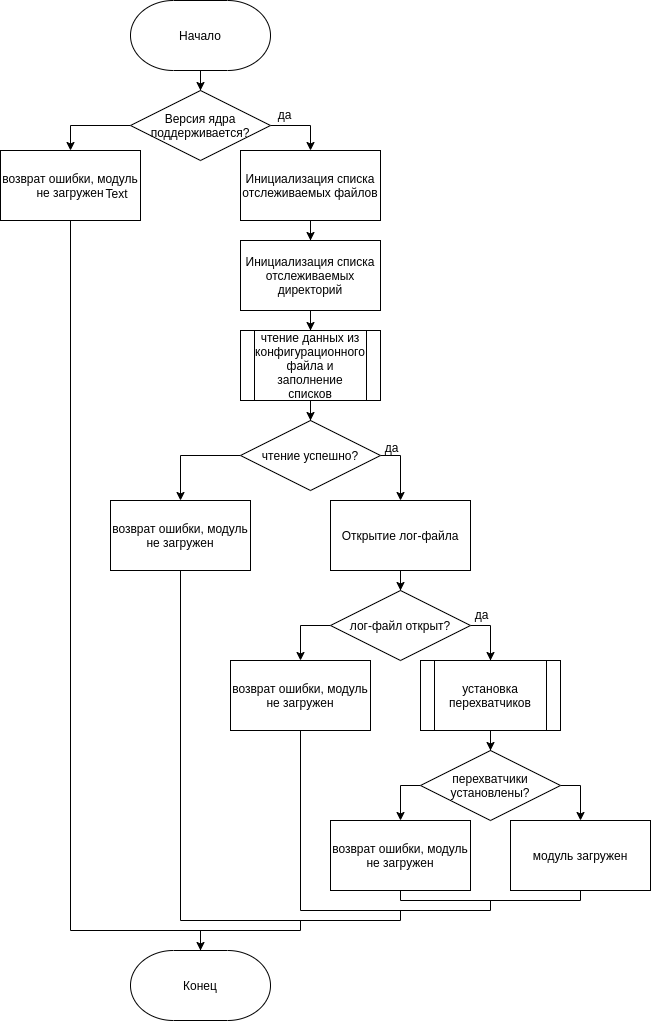
\includegraphics[width=12cm]{img/load}}
    \caption{Схема алгоритма загрузки модуля.}
    \label{fig:load}
\end{figure}

\newpage
\begin{figure}[!h]
    \center{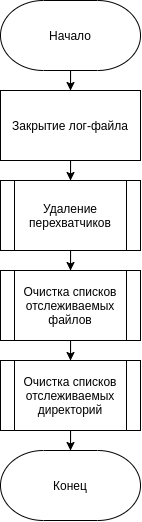
\includegraphics[width=3cm]{img/unload}}
    \caption{Схема алгоритма выгрузки модуля.}
    \label{fig:unload}
\end{figure}

На рисунках \ref{fig:mkdir} приведены схемы наших обработчиков системных вызовов openat(), creat(), write(), unlink(), unlinkat(), mkdir(), mkdirat().

\newpage
\begin{figure}[!h]
    \center{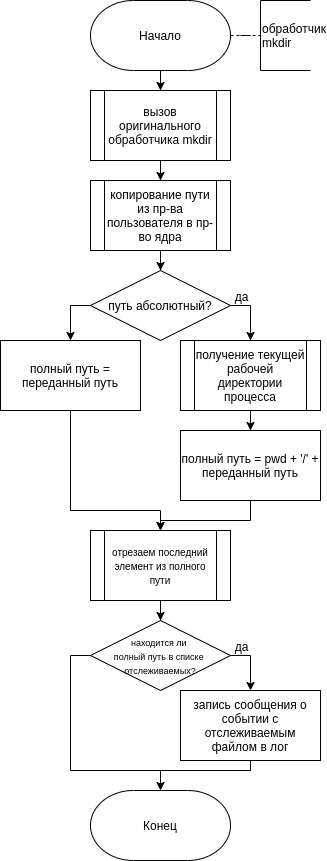
\includegraphics[width=8cm]{img/mkdir}}
    \caption{Наш обработчик mkdir().}
    \label{fig:mkdir}
\end{figure}

\newpage
\begin{figure}[!h]
    \center{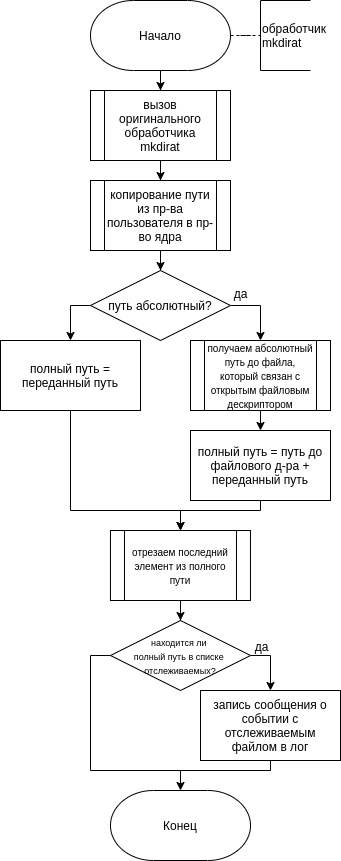
\includegraphics[width=8cm]{img/mkdirat}}
    \caption{Наш обработчик mkdirat().}
    \label{fig:mkdirat}
\end{figure}

\newpage
\begin{figure}[!h]
    \center{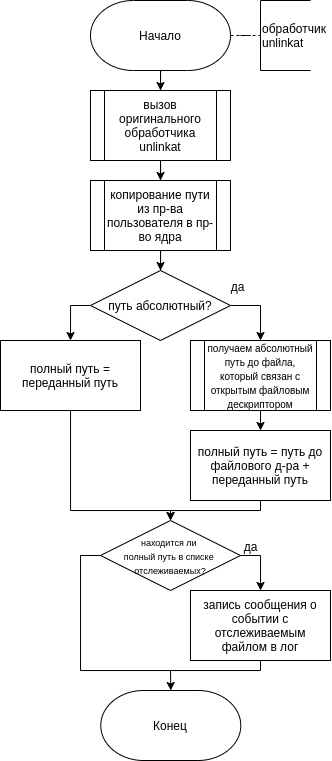
\includegraphics[width=8cm]{img/unlinkat}}
    \caption{Наш обработчик unlinkat().}
    \label{fig:unlinkat}
\end{figure}

\newpage
\begin{figure}[!h]
    \center{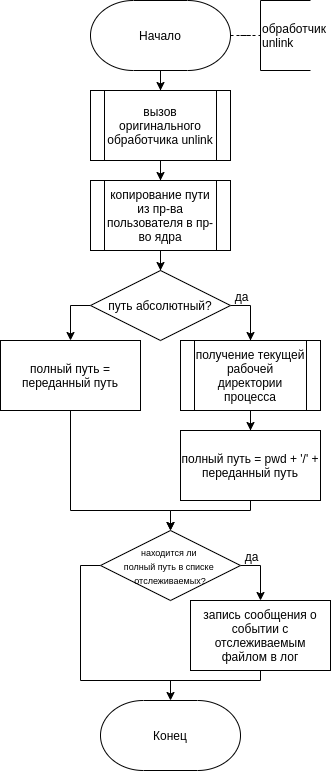
\includegraphics[width=8cm]{img/unlink}}
    \caption{Наш обработчик unlink().}
    \label{fig:unlink}
\end{figure}

\newpage
\begin{figure}[!h]
    \center{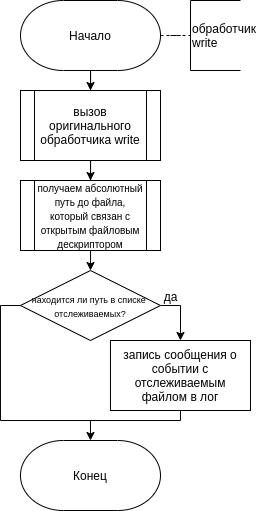
\includegraphics[width=8cm]{img/write}}
    \caption{Наш обработчик write().}
    \label{fig:write}
\end{figure}

\newpage
\begin{figure}[!h]
    \center{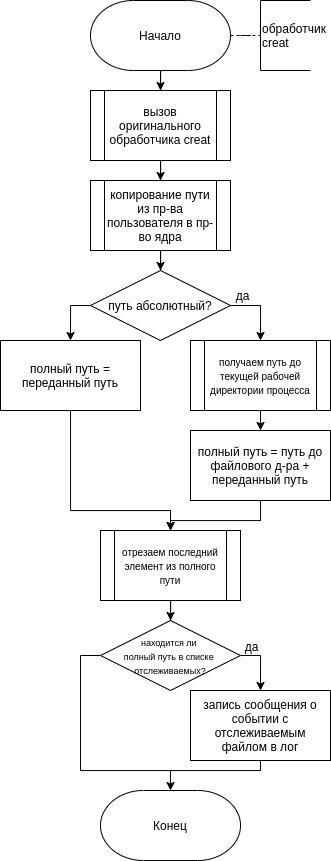
\includegraphics[width=8cm]{img/creat}}
    \caption{Наш обработчик creat().}
    \label{fig:creat}
\end{figure}

\newpage
\begin{figure}[!h]
    \center{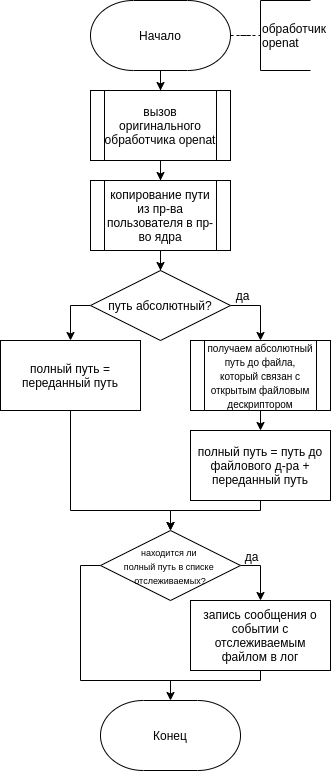
\includegraphics[width=8cm]{img/openat}}
    \caption{Наш обработчик openat().}
    \label{fig:openat}
\end{figure}

\newpage
\section{Технологический раздел раздел}

В данном разделе будет выбран язык и среда программирования, будет приведена реализация наиболее важных функций, будут описаны действия по установке разработанного модуля ядра, а также описано его тестирование.

\subsection{Выбор языка программирования}

В настоящее время операционная система Linux позволяет создавать загружаемые модули ядра на языках C и Rust.

На виртуальной конференции «2020 Linux Plumbers Conference», где ведущие разработчики ядра Linux обсуждают будущее Linux, говорилось о введении Rust в качестве второго языка ядра. Rust – это системный язык программирования высокого уровня, спонсируемый Mozilla, являющейся материнской компанией Firefox.

Однако Rust еще только начал развиваться и не так популярен, как C, поэтому не обладает достаточным количеством документации и примеров. По этой причине для реализации загружаемого модуля ядра был выбран язык C.

\subsection{Выбор среды разработки}

Для написания модуля был выбран редактор Visual Studio Code. Он имеет следующие преимущества:

\begin{itemize}
	\item является «лёгким» редактором кода;
	\item включает в себя отладчик, инструменты для работы с Git, подсветку синтаксиса, IntelliSense,  средства для рефакторинга и навигацию по коду;
	\item имеет широкие возможности для кастомизации: пользовательские темы, сочетания клавиш и файлы конфигурации;
	\item распространяется бесплатно, разрабатывается как программное обеспечение с открытым исходным кодом;
	\item посредством встроенного в продукт пользовательского интерфейса можно загрузить и установить несколько тысяч полезных расширений.
\end{itemize}

\subsection{Взаимодействие с пользователем}

Модуль выводит информацию в системный журнал и в свой лог-файл.

В системный журнал выводятся отладочные сообщения, сообщающие о том, что модуль был загружен или выгружен, либо о том, что произошла ошибка при чтении конфигурационного файла.

В лог-файл выводятся сообщения о событиях, произошедших с отслеживаемыми файлами. Лог-файл создается в каталоге /var/log и имеет имя fsmonitor.log. Таким образом, абсолютный путь до лог-файла -- /var/log/fsmonitor.log.

Информацию о файлах, действия с которыми необходимо отслеживать, модуль считывает из своего конфигурационного файла, который необходимо создать до загрузки модуля.  Конфигурационный файл необходимо создать в каталоге /etc с именем fsmonitor.conf. Таким образом, абсолютный путь до конфигурационного файла -- /etc/fsmonitor.conf.

Формат и создание конфигурационного файла описано далее в этой главе.

\subsection{Ограничения}

Загружаемый модуль был разработан для версий ядра 4.17 - 5.6 и архитектуры x86\_64. Это связано с ограничениями на символ ядра kallsyms\_lookup\_name, который в более поздних версиях ядра перестал быть экспортируемым.

В случае, если в системный вызов передается путь, содержащий <<точки>> (каталоги . и ..), то такие пути модулем не обрабатываются. Даже если такой конечный путь ведет к тому же файлу, что и один из путей в конфигурационном файле, то действия с таким файлом не будут отслежены модулем.

В модуле не реализован механизм очистки или закольцовывания лог-файла, поэтому при больших количествах перехватов его размер может быть значительным. В случае чрезмерного разрастания лог-файла следует выгрузить модуль и загрузить его заново, так как при загрузке модуль очищает лог-файл.

\subsection{Формат конфигурационного файла}

Все пути в конфигурационном файле должны быть абсолютными и начинаться с символа <</>>. Это разделитель пути в операционной системе Linux.

На каждой строке должен располагаться только один путь до одного файла.

Путь не должен заканчиваться символом <</>> (в этом случае возможно некорректное определение, является ли файл отслеживаемым).

При необходимости следить за всеми файлами, можно указать в конфигурационном файле маркер <<ALL>>. Если при чтении конфигурационного файла модуль встречает этот маркер, то, независимо от того, указаны ли там другие пути, он будет производить мониторинг действий с любыми файлами. Следует обратить внимание, что в этом случае лог-файл будет очень быстро увеличиваться в размерах (см. ограничения) из-за того, что перехватываемые системные вызовы вызываются постоянно. Поэтому не рекомендуется использовать маркер ALL.

\subsection{Реализация загружаемого модуля}

Нам потребуется найти и сохранить адрес функции, которую мы будем перехватывать. Ftrace позволяет трассировать функции по имени, но нам всё равно надо знать адрес оригинальной функции, чтобы вызывать её. Добыть адрес можно с помощью kallsyms — списка всех символов в ядре. Поиск адеса функции по ее имени приведен в листинге \ref{lst:resolve}.

\begin{lstlisting}[language=C++,label={lst:resolve}, caption=\text{Поиск адреса функции по ее имени.}]
/**
* fh_resolve_hook_address() - поиск адреса функции, 
* 							   которую будем перехватывать
* @hook: хук, в котором заполнено поле name
*
* @returns 0 в случае успеха, иначе отрицательный код ошибки.
*/
static int fh_resolve_hook_address(struct ftrace_hook *hook)
{
	hook->address = kallsyms_lookup_name(hook->name);
  
	if (!hook->address)
    {
		printk(KERN_INFO "unresolved symbol: %s\n", hook->name);
		return -ENOENT;
    }
  
#if USE_FENTRY_OFFSET
   	*((unsigned long *)hook->original) = hook->address + MCOUNT_INSN_SIZE;
#else
	*((unsigned long *)hook->original) = hook->address;
#endif
   
   return 0;
}
\end{lstlisting}

Дальше необходимо инициализировать структуру ftrace\_ops. В ней обязательным
полем является лишь func, указывающая на коллбек, но нам также необходимо
установить некоторые важные флаги (листинг \ref{lst:ops}). fh\_ftrace\_thunk() — это наш коллбек, который ftrace будет вызывать при трассировании функции. Флаги, которые мы устанавливаем, будут необходимы для выполнения перехвата. Они предписывают ftrace сохранить и восстановить регистры процессора, содержимое которых мы сможем изменить в коллбеке.

Для включения перехвата необходимо сначала включить ftrace для интересующей нас функции с помощью ftrace\_set\_filter\_ip(), а затем разрешить ftrace вызывать наш коллбек с помощью register\_ftrace\_function(). Защита ftrace от рекурсии бесполезна, если изменять \%rip, поэтому вычлючаем ее с помощью RECURSION\_SAFE. Проверки для защиты от рекурсии будут выполнены на входе в трассируемую функцию.


\begin{lstlisting}[language=C++,label={lst:ops}, caption=\text{Инициализация структуры ftrace\_ops.}]
/**
* fh_install_hook() - регистрация и активация хука
* @hook: хук для установки
*
* @returns 0 в случае успеха, иначе отрицательный код ошибки.
*/
int fh_install_hook(struct ftrace_hook *hook)
{
   int err;
   
   err = fh_resolve_hook_address(hook);
   if (err)
	   return err;

    hook->ops.func = fh_ftrace_thunk;
    hook->ops.flags = FTRACE_OPS_FL_SAVE_REGS | FTRACE_OPS_FL_RECURSION_SAFE | FTRACE_OPS_FL_IPMODIFY;

    err = ftrace_set_filter_ip(&hook->ops, hook->address, 0, 0);
    if (err)
    {
	    printk(KERN_INFO "ftrace_set_filter_ip() failed: %d\n", err);
	    return err;
    }

    err = register_ftrace_function(&hook->ops);
    if (err)
    {
	    printk(KERN_INFO "register_ftrace_function() failed: %d\n",err);
	    ftrace_set_filter_ip(&hook->ops, hook->address, 1, 0);
	    return err;
    }
    return 0;
}
\end{lstlisting}

Выключается перехват аналогично, только в обратном порядке (листинг \ref{lst:off}). После завершения вызова unregister\_ftrace\_function() гарантируется отсутствие активаций установленного коллбека в системе (а вместе с ним — и наших обёрток). Поэтому мы можем спокойно выгрузить модуль-перехватчик, не опасаясь, что где-то в системе ещё выполняются наши функции.

\begin{lstlisting}[language=C++,label={lst:off}, caption=\text{Выключение перехвата.}]
/**
* fh_remove_hook() - выключить хук
* @hook: хук для выключения
*/
void fh_remove_hook(struct ftrace_hook *hook)
{
	int err;

	err = unregister_ftrace_function(&hook->ops);
	if (err)
	{
		printk(KERN_INFO "unregister_ftrace_function() failed: %d\n", err);
	}
   
	err = ftrace_set_filter_ip(&hook->ops, hook->address, 1, 0);
	if (err)
	{
		printk(KERN_INFO "ftrace_set_filter_ip() failed: %d\n", err);
    }
}
\end{lstlisting}

Ftrace позволяет изменять состояние регистров после выхода из коллбека. Изменяя регистр \%rip — указатель на следующую исполняемую инструкцию,— мы изменяем инструкции, которые исполняет процессор — то есть можем заставить его выполнить безусловный переход из текущей функции в нашу. Таким образом мы перехватываем управление на себя.

Коллбек для ftrace выглядит следующим образом (листинг \ref{lst:callback}). С помощью макроса container\_of() мы получаем адрес нашей struct ftrace\_hook по адресу внедрённой в неё struct ftrace\_ops, после чего заменяем значение регистра \%rip в структуре struct pt\_regs на адрес нашего обработчика. Спецификатором notrace необходимо помечать функции, запрещённые для трассировки с помощью ftrace. Это помогает предотвратить зависание системы в бесконечном цикле при трассировании всех функций в ядре.

Когда наша обёртка вызовет оригинальную функцию, та опять попадёт в ftrace, который опять вызовет наш коллбек, который опять передаст управление обёртке. Эту бесконечную рекурсию необходимо оборвать. Для этого используется parent\_ip -- один из аргументов ftrace-коллбека, который содержит адрес возврата в функцию, которая вызвала трассируемую функцию. Мы же можем воспользоваться им для того, чтобы отличить первый вызов перехваченной функции от повторного. При повторном вызове parent\_ip должен указывать внутрь нашей обёртки, тогда как при первом — куда-то в другое место ядра. Проверку на вхождение можно очень эффективно выполнить, сравнивая адрес с границами текущего модуля (который содержит все наши функции). 

\begin{lstlisting}[language=C++,label={lst:callback}, caption=\text{Обратный вызов для ftrace.}]
static void notrace fh_ftrace_thunk(unsigned long ip, unsigned long arent_ip, struct ftrace_ops *ops, struct pt_regs *regs)
{
	struct ftrace_hook *hook = container_of(ops, struct ftrace_hook, ops);

#if USE_FENTRY_OFFSET
	regs->ip = (unsigned long)hook->function;
#else
	if (!within_module(parent_ip, THIS_MODULE))
	regs->ip = (unsigned long)hook->function;
#endif
}
\end{lstlisting}

Функция-обёртка, которая вызывается позже, будет выполняться в том же контексте, что и оригинальная функция. Поэтому там можно делать то же, что позволено делать в перехватываемой функции.

Пути к отслеживаемым файлам хранятся в двух списувх -- списке файлов и списке директорий. Структуры, описывающие такие списки, приведены в листинге \ref{lst:lists}.


\begin{lstlisting}[language=C++,label={lst:lists}, caption=\text{Реализация списка.}]
struct list_node
{
	struct list_node *next_node;
	void *value;
	size_t type_size;
};

struct list
{
	struct list_node *head;
	struct list_node *tail;
};
\end{lstlisting}

Функции загрузки и выгрузки модуля, а также список всех перехватываемых системных вызовов, представлены в листинге \ref{lst:init}

\begin{lstlisting}[language=C++,label={lst:init}, caption=\text{Загрузка и выгрузка модуля.}]
static struct ftrace_hook fs_hooks[] = {
	HOOK("sys_mkdir", fh_sys_mkdir, &real_sys_mkdir),
	HOOK("sys_openat", fh_sys_openat, &real_sys_openat),
	HOOK("sys_creat", fh_sys_creat, &real_sys_creat),
	HOOK("sys_unlink", fh_sys_unlink, &real_sys_unlink),
	HOOK("sys_write", fh_sys_write, &real_sys_write),
	HOOK("sys_unlinkat", fh_sys_unlinkat, &real_sys_unlinkat),
	HOOK("sys_mkdirat", fh_sys_mkdirat, &real_sys_mkdirat)
};

static int fh_init(void)
{
	int err;
	pr_info("============");
#ifndef PTREGS_SYSCALL_STUBS
	pr_info("Kernel version is not supported\n");
	return -1;
#else

	init(&monitor_dirs);
	init(&monitor_files);
	if ((err = read_config()) != 0)
	{
		if (err == -1)
			pr_info("Unable to read config file\n");
		if (err == -2)
			pr_info("Invalid config file format\n");
		if (err == -3)
			pr_info("Files writen in config do not exist\n");
		return err;
	}

	f = filp_open(LOG_FILE, O_CREAT | O_TRUNC | O_WRONLY | O_LARGEFILE, 0);
	if (IS_ERR(f))
	{
		pr_info("Unable to open log file\n");
		return -1;
	}
	pr_info("Log file opened\n");

	err = fh_install_hooks(fs_hooks, ARRAY_SIZE(fs_hooks));
	if (err)
	{
		free_list(&monitor_dirs);
		free_list(&monitor_files);
	    pr_info("Unable to install hooks\n");
		return err;
	}

	pr_info("Module loaded\n");

	return 0;
#endif
}
module_init(fh_init);

static void fh_exit(void)
{
	filp_close(f, NULL);
	pr_info("Log file closed\n");
	fh_remove_hooks(fs_hooks, ARRAY_SIZE(fs_hooks));
	pr_info("Hooks removed\n");
	free_list(&monitor_dirs);
	free_list(&monitor_files);
	pr_info("Lists cleared\n");
	pr_info("Module unloaded\n");
}
module_exit(fh_exit);
\end{lstlisting}

Нам также необходимо отключить оптимизацию хвостовых вызовов (tail call optimization) с помощью директивы pragma (листинг \ref{lst:tail}). Она позволяет компилятору заменить честный вызов функции на прямой переход к её телу, если одна функция вызывает другую и сразу же возвращает её значение. 

Оптимизация хвостовых вызовов позволяет сэкономить немного времени на формировании стекового фрейма, в который входит и адрес возврата, сохраняемый в стеке инструкцией CALL. Однако, для нас корректность адреса возврата играет критичную роль — мы используем parent\_ip для принятия решения о перехвате. После оптимизации функция наши функции-обработчики больше не сохраняют новый адрес возврата на стеке, там остаётся старый — указывающий в ядро. Поэтому parent\_ip продолжает указывать внутрь ядра, что и приводит в конечном итоге к образованию бесконечного цикла.


\begin{lstlisting}[language=C++,label={lst:tail}, caption=\text{Отключение оптимизации хвостовых вызовов.}]
#pragma GCC optimize("-fno-optimize-sibling-calls")
\end{lstlisting}


Полная реализация модуля представлена в приложении А.

\subsection{Сборка и установка модуля}

Сборка модуля производится с помощью утилиты make. Makefile приведен в листинге \ref{lst:make}.

\begin{lstlisting}[language=C++,label={lst:make}, caption=\text{Makefile.}]
CURRENT = $(shell uname -r)
KDIR = /lib/modules/$(CURRENT)/build
PWD = $(shell pwd)
TARGET = fsmonitor
	
obj-m := $(TARGET).o 
	
default:
	$(MAKE) -I /usr/include/x86_64-linux-gnu -C $(KDIR) M=$(PWD) modules
	make clean
clean:
	@rm -f *.o .*.cmd .*.flags *.mod.c *.order *.mod
	@rm -fR .tmp*
	@rm -rf .tmp_versions
disclean: clean
	@rm *.ko *.symvers
\end{lstlisting}

Перед установкой модуля необходимо создать конфигурационный файл модуля командой \textit{sudo touch /etc/fsmonitor.conf}. Для записи необходимых путей в конфигурационный файл необходимо запустить текстовый редактор с привелегиями суперпользователя и открыть конфигурационный файл. 

После сборки и создания конфигурационного файла, необходимо загрузить модуль в ядро командой \textit{sudo insmod fsmonitor.ko}. В случае, если конфигурационный файл был успешно прочитан, модуль будет загружен в ядро. Для проверки, что модуль загружен, можно использовать команду \textit{lsmod | grep fsmonitor}. Если же во время чтения конфигурационного файла произошла ошибка, модуль не будет загружен.

Проверить сообщения от модуля в системном журнале можно с помощью команды \textit{sudo dmesg | grep ftrace\_hook}. Проверить сообщения от модуля в лог-файле можно командой \textit{sudo cat /var/log/fsmonitor.log}.

Для выгрузки модуля из ядра необходимо выполнить команду \textit{sudo rmmod fsmonitor}.

При изменении конфигурационного файла необходимо выгрузить модуль, если он загружен, и загрузить его в ядно заново.

В случае успешной загрузки модуля в системный журнал будет выведено сообщение <<Module loaded>>. В случае успешной выгрузки модуля в системный журнал будет выведено сообщение <<Module unloaded>>.

\subsection{Возможные ошибки при загрузке модуля}

При загрузке модуля могут возникнуть следующие ошибки:

\begin{itemize}
	\item версия ядра не поддерживается;
	\item ошибка чтения конфигурационного файла;
	\item ошибка открытия лог-файла;
	\item ошибка при установке перехватчиков.
\end{itemize}

При чтении конфигурационного файла могут произойти следующие ошибки:

\begin{itemize}
	\item конфигурационного файла не существует (он не был создан до загрузки модуля или был удален). В этом случае в системном журнале появится сообщение <<Unable to read config file>>;
	\item неверный формат записей в конфигурационном файле. В этом случае в системном журнале появится сообщение <<Invalid config file format>>;
	\item файлов, указанных в конфигурационном файле, не существует. В этом случае в системном журнале появится сообщение <<Files writen in config do not exist>>.
\end{itemize}

При ошибке чтения конфигурационного файла необходимо проверить наличие файла и корректность указанных там путей, после чего снова загрузить модуль.

При ошибке открытия лог-файла в системный журнал будет выведено сообщени <<Unable to open log file>>.

При ошибке установки перехватчиков в системный журнал будет выведено сообщени <<Unable to install hooks>>.

\subsection{Тестирование разработанного модуля}

Отладка и тестирование в ядре Linux -- довольно сложная задача, так как единственным способом взаимодействия ядра с пользователем являются различные лог-файлы или системный журнал. В связи с этим было проведено ручное тестирование разработанного модуля ядра. На каждом шаге был установлен отладочный вывод сообщений в системный журнал и контролировалась их корректность.

С учетом изложенных выше ограничений на работу разработанного модуля, тестирование было пройдено.

\newpage
\section*{Заключение}
\addcontentsline{toc}{section}{Заключение}

В данной работе были выполнены следующие задачи.

\begin{enumerate}
	\item Были проанализированы возможные способы перехвата системных вызовов и выбран наиболее подходящий -- ftrace.
	\item Был изучен алгоритм перехвата системных вызовов с использованием ftrace.
	\item Был реализован загружаемый модуль ядра, перехватывающий системные вызовы openat(), creat(), write(), unlink(), unlinkat(), mkdir(), mkdirat().
	\item Было проведено ручное тестирование разработанного модуля. Тесты были пройдены.
\end{enumerate}

Таким образом, поставленная цель была достигнута.



\newpage
\begin{thebibliography}{3}
\addcontentsline{toc}{section}{Список литературы}

\bibitem{zirulnik}
Цилюрик О.И. Модули ядра Linux. Модификация системных вызовов. [Электронный ресурс]. -- Режим доступа: http://rus-linux.net/MyLDP/BOOKS/Moduli-yadra-Linux/08/kern-mod-08-04.html, свободный -- (27.11.2020).

\bibitem{lsm_1}
Linux Security Modules: General Security Hooks for Linux [Электронный ресурс]. -- Режим доступа: https://www.kernel.org/doc/html/latest/security/lsm.html, свободный -- (27.11.2020).

\bibitem{lsm_2}
Linux Security Modules:
General Security Support for the Linux Kernel [Электронный ресурс]. -- Режим доступа: https://www.usenix.org/legacy/events/sec02/full\_papers/wright/wright\_html/in-dex.html, свободный -- (27.11.2020).

\bibitem{syscall_man}
syscalls(2) — Linux manual page. -- Режим доступа: https://man7.org/linux/man-pages/man2/syscalls.2.html, свободный -- (27.11.2020).

\bibitem{kprobes}
Kernel Probes (Kprobes). -- Режим доступа: https://www.kernel.org/doc/Documentation/kprobes.txt, свободный -- (28.11.2020).

\bibitem{kprobes_ibm}
Kernel debugging with Kprobes. -- Режим доступа: https://www.ibm.com/developerworks/library/l-kprobes/index.html, свободный -- (28.11.2020).

\bibitem{ftrace}
Перехват функций в ядре Linux с помощью ftrace: https://habr.com/ru/post/413241/, свободный -- (28.11.2020).

\bibitem{lkmj}
Loadable Kernel Module Programming and System Call Interception: https://www.linuxjournal.com/article/4378, свободный -- (28.11.2020).

\bibitem{ftrace_kern}
ftrace - Function Tracer: https://www.kernel.org/doc/html/latest/trace/ftrace.html, свободный -- (28.11.2020).


\bibitem{bootlin}
Bootlin: https://elixir.bootlin.com, свободный -- (18.12.2020).

\bibitem{proc}
proc: https://www.opennet.ru/man.shtml?topic=proc\&category=5\&russian=0, свободный -- (18.12.2020).

\bibitem{proc}
Что нового в ядре Linux: https://habr.com/ru/post/520950/, свободный -- (21.12.2020).

\end{thebibliography}

\newpage
\appendix
\section*{Приложение А}
\addcontentsline{toc}{section}{Приложение А}

\begin{lstlisting}[language=C++,label={lst:ftrace_hook}]
#define pr_fmt(fmt) "ftrace_hook: " fmt

#include <linux/ftrace.h>
#include <linux/kallsyms.h>
#include <linux/kernel.h>
#include <linux/linkage.h>
#include <linux/module.h>
#include <linux/slab.h>
#include <linux/uaccess.h>
#include <linux/version.h>
#include <linux/fs.h>
#include <linux/fs_struct.h>
#include <linux/timekeeping.h>
#include <linux/stat.h>
#include <linux/types.h>
#include <linux/dcache.h>
#include <asm/segment.h>
#include <linux/buffer_head.h>
#include <linux/fdtable.h>

MODULE_DESCRIPTION("File system monitor");
MODULE_AUTHOR("Ovchinnikova Anastasia");
MODULE_LICENSE("GPL");

/*
 * There are two ways of preventing vicious recursive loops when hooking:
 * - detect recusion using function return address (USE_FENTRY_OFFSET = 0)
 * - avoid recusion by jumping over the ftrace call (USE_FENTRY_OFFSET = 1)
 */
#define USE_FENTRY_OFFSET 0

/**
 * struct ftrace_hook - описывает перехватываемую функцию
 *
 * @name:       имя перехватываемой функции
 *
 * @function:   адрес функции-обёртки, которая будет вызываться вместо
 *              перехваченной функции
 *
 * @original:   указатель на место, куда следует записать адрес
 *              перехватываемой функции, заполняется при установке
 *
 * @address:    адрес перехватываемой функции, выясняется при установке
 *
 * @ops:        служебная информация ftrace, инициализируется нулями,
 *              при установке перехвата будет доинициализирована
 */
struct ftrace_hook
{
	const char *name;
	void *function;
	void *original;

	unsigned long address;
	struct ftrace_ops ops;
};

#define LOG_FILE "/var/log/fsmonitor.log"
#define CONFIG_PATH "/etc/fsmonitor.conf"
#define BUFF_SIZE 1024 //PATH_MAX
#define MONITOR_ALL_MARKER "ALL"

struct list_node
{
	struct list_node *next_node;
	void *value;
	size_t type_size;
};

struct list
{
	struct list_node *head;
	struct list_node *tail;
};

short Monitor_All = 0;
struct file *f;
struct list monitor_files, monitor_dirs;
loff_t File_Pos = 0;

/**
 * инициализация списка
 */
void init(struct list *lst)
{
	lst->head = NULL;
	lst->tail = NULL;
}

/**
 * добавление элемента в список
 */
struct list_node *push(struct list *node, void *value, size_t size)
{
	void *next_node = kmalloc(sizeof(struct list_node) + size, GFP_KERNEL);
	struct list_node *__next_node = next_node;
	__next_node->value = next_node + sizeof(struct list_node);
	__next_node->type_size = size;
	__next_node->next_node = NULL;
	memcpy(__next_node->value, value, size);

	if (node->head == NULL)
	{
		node->head = __next_node;
		node->tail = __next_node;
	}
	else
	{
		node->tail->next_node = __next_node;
		node->tail = __next_node;
	}

	return next_node;
}

/*
 * удаление элемента из списка
 */
struct list_node *pop(struct list *node)
{
	struct list_node *value = node->head == NULL
								  ? NULL
								  : node->head->next_node;

	if (value != NULL)
	{
		kfree(node->head);
		node->head = value;
	}
	return value;
}

/**
 * очищение списка
 */ 
void free_list(struct list *list)
{
	if (list->head != NULL)
	{
		do
		{
			//pr_info("Deleting %s\n", *(char **)list->head->value);
			kfree(*(char **)list->head->value);
		} while (pop(list) != NULL);
	}
}

/**
 * удаляет последний элемент пути (path/to/file -> path/to)
 */
char *cut_last_filename(char *filename)
{
	size_t n;
	int i = 0, go = 1;
	n = strlen(filename);
	for (i = n - 1; i >= 0 && go == 1; --i)
	{
		if (filename[i] == '/')
		{
			go = 0;
		}
		filename[i] = '\0';
	}
	return filename;
}

int write_log(const char *log)
{
	time64_t cur_seconds;
	unsigned long local_time;
	char *new_sl;
	int ret;

	new_sl = kmalloc(BUFF_SIZE, GFP_KERNEL);
	if (new_sl == NULL)
	{
		pr_info("Unable to allocate memory\n");
		return -1;
	}

	if (log == NULL)
	{
		pr_info("Empty log message.\n");
		return -1;
	}

	if (IS_ERR(f))
	{
		pr_info("Failed to write log");
		return -1;
	}

	cur_seconds = ktime_get_real_seconds();
	local_time = (u32)(cur_seconds - (sys_tz.tz_minuteswest * 60));

	snprintf(new_sl, BUFF_SIZE, "%.2lu:%.2lu:%.6lu \t %s",
			 (local_time / 3600) % (24),
			 (local_time / 60) % (60),
			 local_time % 60,
			 log);

	ret = kernel_write(f, new_sl, strlen(new_sl), &File_Pos);
	File_Pos += strlen(new_sl);
	kfree(new_sl);

	return 0;
}

/**
 * проверяет, содержит ли список имя name
 * @returns 1 если да, иначе 0 
 */
int list_find(struct list *list, const char *name)
{
	struct list_node *_node = list->head;
	int ret = 0;
	while (_node != NULL && ret == 0)
	{
		if (strcmp(name, *(char **)_node->value) == 0)
		{
			ret = 1;
		}
		_node = _node->next_node;
	}
	return ret;
}

/**
 * проверяет, находится ли данный файл в списке отслеживаемых
 * @returns 1 если да, иначе 0 
 */
int check_filename(const char *filename, int search_file, int search_dir)
{
	int ret = 0;

	if (search_file == 1 && search_dir == 0)
	{
		ret = list_find(&monitor_files, filename);
		return ret;
	}
	if (search_dir == 1 && search_file == 0)
	{
		ret = list_find(&monitor_dirs, filename);
		return ret;
	}
	if (search_file == 1 && search_dir == 1)
	{
		ret = list_find(&monitor_files, filename);
		ret += list_find(&monitor_dirs, filename);
		if (ret == 2)
		{
			ret--;
		}
		return ret;
	}
	return ret;
}

/**
 * fh_resolve_hook_address() - поиск адреса функции, 
 * 							   которую будем перехватывать
 * @hook: хук, в котором заполнено поле name
 *
 * @returns 0 в случае успеха, иначе отрицательный код ошибки.
 */
static int fh_resolve_hook_address(struct ftrace_hook *hook)
{
	hook->address = kallsyms_lookup_name(hook->name);

	if (!hook->address)
	{
		printk(KERN_INFO "unresolved symbol: %s\n", hook->name);
		return -ENOENT;
	}

#if USE_FENTRY_OFFSET
	*((unsigned long *)hook->original) = hook->address + MCOUNT_INSN_SIZE;
#else
	*((unsigned long *)hook->original) = hook->address;
#endif

	return 0;
}

/**
 *	fh_ftrace_thunk() -- обратный вызов, который будет вызываться 
 						 при трассировании функции
 * Изменяя регистр %rip -- указатель на следующую исполняемую 
 * инструкцию,-- мы изменяем инструкции, которые исполняет процессор 
 * -- то есть можем заставить его выполнить безусловный переход из 
 * текущей функции в нашу. Таким образом мы перехватываем 
 * управление на себя.
 * notrace помогает предотвратить зависание системы в бесконечном цикле
 */
static void notrace fh_ftrace_thunk(unsigned long ip, unsigned long parent_ip,
									struct ftrace_ops *ops, struct pt_regs *regs)
{
	// получаем адрес нашей struct ftrace_hook
	// по адресу внедрённой в неё struct ftrace_ops
	struct ftrace_hook *hook = container_of(ops, struct ftrace_hook, ops);

	// заменяем значение регистра %rip в структуре
	// struct pt_regs на адрес нашего обработчика
#if USE_FENTRY_OFFSET
	regs->ip = (unsigned long)hook->function;
#else
	// parent_ip содержит адрес возврата в функцию,
	// которая вызвала трассируемую функцию
	// можно воспользоваться им для того,
	// чтобы отличить первый вызов перехваченной функции от повторного
	if (!within_module(parent_ip, THIS_MODULE))
		regs->ip = (unsigned long)hook->function;
#endif
}

/**
 * fh_install_hook() - регистрация и активация хука
 * @hook: хук для установки
 *
 * @returns 0 в случае успеха, иначе отрицательный код ошибки.
 */
int fh_install_hook(struct ftrace_hook *hook)
{
	int err;

	err = fh_resolve_hook_address(hook);
	if (err)
		return err;

	/*
	 * Мы будем модифицировать регистр %rip поэтому необходим флаг IPMODIFY
	 * и SAVE_REGS. Флаги предписывают ftrace сохранить и восстановить
	 * регистры процессора, содержимое которых мы сможем изменить в 
	 * коллбеке. Защита ftrace от рекурсии бесполезна, если 
	 * изменять %rip, поэтому вычлючаем ее с помощью RECURSION_SAFE.
	 * Проверки для защиты от рекурсии будут выполнены на входе в
	 * трассируемую функцию.
	 */
	hook->ops.func = fh_ftrace_thunk;
	hook->ops.flags = FTRACE_OPS_FL_SAVE_REGS | FTRACE_OPS_FL_RECURSION_SAFE | FTRACE_OPS_FL_IPMODIFY;

	// включить ftrace для интересующей нас функции
	err = ftrace_set_filter_ip(&hook->ops, hook->address, 0, 0);
	if (err)
	{
		printk(KERN_INFO "ftrace_set_filter_ip() failed: %d\n", err);
		return err;
	}

	// разрешить ftrace вызывать наш коллбек
	err = register_ftrace_function(&hook->ops);
	if (err)
	{
		printk(KERN_INFO "register_ftrace_function() failed: %d\n", err);
		// выключаем ftrace в случае ошибки
		ftrace_set_filter_ip(&hook->ops, hook->address, 1, 0);
		return err;
	}

	return 0;
}

/**
 * fh_remove_hook() - выключить хук
 * @hook: хук для выключения
 */
void fh_remove_hook(struct ftrace_hook *hook)
{
	int err;

	// отключаем наш коллбек
	err = unregister_ftrace_function(&hook->ops);
	if (err)
	{
		printk(KERN_INFO "unregister_ftrace_function() failed: %d\n", err);
	}

	// отключаем ftrace
	err = ftrace_set_filter_ip(&hook->ops, hook->address, 1, 0);
	if (err)
	{
		printk(KERN_INFO "ftrace_set_filter_ip() failed: %d\n", err);
	}
}

/**
 * fh_install_hooks() - регистрация хуков
 * @hooks: массив хуков для регистрации
 * @count: количество хуков для регистрации
 *
 * Если один из хуков не удалось зарегистрировать, 
 * то все остальные (которые удалось установить), удаляются.
 *
 * @returns 0 в случае успеха, иначе отрицательный код ошибки.
 */
int fh_install_hooks(struct ftrace_hook *hooks, size_t count)
{
	int err = 0;
	size_t i;

	for (i = 0; i < count && err == 0; i++)
	{
		err = fh_install_hook(&hooks[i]);
	}
	if (err == 0)
	{
		return 0;
	}
	while (i != 0)
	{
		fh_remove_hook(&hooks[--i]);
	}

	return err;
}

/**
 * fh_remove_hooks() - выключить хуки
 * @hooks: массив хуков для выключения
 * @count: количество хуков для выключения
 */
void fh_remove_hooks(struct ftrace_hook *hooks, size_t count)
{
	size_t i;

	for (i = 0; i < count; i++)
		fh_remove_hook(&hooks[i]);
}

#ifndef CONFIG_X86_64
#error Currently only x86_64 architecture is supported
#endif

#if defined(CONFIG_X86_64) &&                           \
	(LINUX_VERSION_CODE >= KERNEL_VERSION(4, 17, 0)) && \
	(LINUX_VERSION_CODE <= KERNEL_VERSION(5, 6, 0))
#define PTREGS_SYSCALL_STUBS 1
#endif

/*
 * Оптимизация хвостового вызова может помешать обнаружению рекурсии
 * на основе обратного адреса в стеке. 
 * Отключаем ее, чтобы предотвратить зависание.
 */
#if !USE_FENTRY_OFFSET
#pragma GCC optimize("-fno-optimize-sibling-calls")
#endif

/**
 * копирование имени файла из пользовательского пространства в пространство ядра
 */ 
static char *duplicate_filename(const char __user *filename)
{
	char *kernel_filename;
	int res;

	if (filename == NULL)
	{
		pr_info("Filename is null\n");
		return NULL;
	}

	kernel_filename = kmalloc(BUFF_SIZE, GFP_KERNEL);
	if (!kernel_filename)
	{
		pr_info("kmalloc() failed\n");
		return NULL;
	}

	if ((res = strncpy_from_user(kernel_filename, filename, BUFF_SIZE)) < 0)
	{
		pr_info("strncpy_from_user() failed: %d \n", res);
		kfree(kernel_filename);
		return NULL;
	}

	return kernel_filename;
}

//asmlinkage long sys_open(const char __user *filename,
//				int flags, umode_t mode);

// настоящий обработчик системного вызова openat
static asmlinkage long (*real_sys_openat)(struct pt_regs *regs);

// обработчик системного вызова openat
static asmlinkage long fh_sys_openat(struct pt_regs *regs)
{
	int ret;
	char *kernel_filename;
	char *proc_filename;
	char *buffer;
	int fd;
	char *full_filename;

	ret = real_sys_openat(regs);
	fd = (long)(void *)regs->di;

	// копируем имя директории из пространства пользователя в пространство ядра
	kernel_filename = duplicate_filename((void *)regs->si);
	if (kernel_filename == NULL)
	{
		pr_info("Unable to duplicate filename\n");
		return ret;
	}

	proc_filename = kmalloc(BUFF_SIZE, GFP_KERNEL);
	buffer = kmalloc(BUFF_SIZE, GFP_KERNEL);
	full_filename = kmalloc(BUFF_SIZE, GFP_KERNEL);
	if (proc_filename == NULL || buffer == NULL || full_filename == NULL)
	{
		pr_info("Unable to allocate memory\n");
		kfree(kernel_filename);
		if (proc_filename != NULL) kfree(proc_filename);
		if (buffer != NULL) kfree(buffer);
		if (full_filename != NULL) kfree(full_filename);
		return ret;
	}

	// если путь не является абсолютным, получаем абсолютный путь до файла, который связан с открытым файловым дескриптором
	if (fd != AT_FDCWD && kernel_filename[0] != '/')
	{
		char *path;
		struct path pwd;
		char *pwd_buff;
		struct file *_file;

		snprintf(proc_filename, BUFF_SIZE, "/proc/%d/fd/%d", current->pid, fd);
		_file = filp_open(proc_filename, 0, 0);

		pwd_buff = kmalloc(BUFF_SIZE, GFP_KERNEL);
		if (pwd_buff == NULL)
		{
			pr_info("Unable to allocate memory\n");
			kfree(kernel_filename);
			kfree(proc_filename);
			kfree(full_filename);
			kfree(buffer);
			return ret;
		}
		pwd = _file->f_path;
		path_get(&pwd);
		path = d_path(&pwd, pwd_buff, BUFF_SIZE);
		kfree(pwd_buff);

		full_filename = strcat(full_filename, path);
		full_filename = strcat(full_filename, "/");
		full_filename = strcat(full_filename, kernel_filename);
	}
	else // путь абсолютный, ничего делать не надо
	{
		full_filename = strcpy(full_filename, kernel_filename);
	}

	// проверяем, находится ли файл или директория в списке отслеживаемых
	if (check_filename(full_filename, 1, 1) == 1)
	{
		char *buff = kmalloc(BUFF_SIZE * 2, GFP_KERNEL);
		if (buff == NULL)
		{
			pr_info("Unable to allocate memory\n");
			kfree(kernel_filename);
			kfree(proc_filename);
			kfree(full_filename);
			kfree(buffer);
			return ret;
		}
		snprintf(buff, BUFF_SIZE * 2, "Process %d OPENAT '%s'. Syscall returned %d\n",
				 current->pid, full_filename, ret);
		write_log(buff);
		kfree(buff);
	}

	kfree(kernel_filename);
	kfree(proc_filename);
	kfree(full_filename);
	kfree(buffer);

	return ret;
}

//static asmlinkage long (*real_sys_creat)(const char __user *pathname, umode_t mode);
// настоящий обработчик системного вызова creat
static asmlinkage long (*real_sys_creat)(struct pt_regs *regs);

// обработчик системного вызова creat
static asmlinkage long fh_sys_creat(struct pt_regs *regs)
{
	int ret;
	char *kernel_filename;
	char *full_filename;
	char *path;
	struct path pwd;
	char *pwd_buff;

	ret = real_sys_creat(regs);

	// копируем имя директории из пространства пользователя в пространство ядра
	kernel_filename = duplicate_filename((void *)regs->di);
	if (kernel_filename == NULL)
	{
		pr_info("Unable to duplicate filename\n");
		return ret;
	}

	// получаем путь до текущей рабочей директории процесса
	pwd_buff = kmalloc(BUFF_SIZE, GFP_KERNEL);
	full_filename = kmalloc(BUFF_SIZE, GFP_KERNEL);
	if (pwd_buff == NULL || full_filename == NULL)
	{
		pr_info("Unable to allocate memory\n");
		kfree(kernel_filename);
		if (pwd_buff != NULL) kfree(pwd_buff);
		if (full_filename != NULL) kfree(full_filename);
		return ret;
	}

	pwd = current->fs->pwd;
	path_get(&pwd);
	path = d_path(&pwd, pwd_buff, BUFF_SIZE);

	if (kernel_filename[0] != '/')
	{
		full_filename = strcat(full_filename, path);
		full_filename = strcat(full_filename, "/");
		full_filename = strcat(full_filename, kernel_filename);
	}
	else
	{
		full_filename = strcpy(full_filename, kernel_filename);
	}
	full_filename = cut_last_filename(full_filename);

	// проверяем, находится ли файл или директория в списке отслеживаемых
	if (check_filename(full_filename, 0, 1) == 1)
	{
		char *buff = kmalloc(BUFF_SIZE * 2, GFP_KERNEL);
		if (buff == NULL)
		{
			pr_info("Unable to allocate memory\n");
			kfree(kernel_filename);
			kfree(full_filename);
			kfree(pwd_buff);
			return ret;
		}
		snprintf(buff, BUFF_SIZE * 2, "Process %d CREAT '%s' at '%s'. Syscall returned %d\n",
				 current->pid, kernel_filename, full_filename, ret);
		write_log(buff);
		kfree(buff);
	}

	kfree(kernel_filename);
	kfree(full_filename);
	kfree(pwd_buff);

	return ret;
}

//static asmlinkage long (*real_sys_write)(unsigned int fd, const char __user *buf,
//										 size_t count);
// настоящий обработчик системного вызова write
static asmlinkage long (*real_sys_write)(struct pt_regs *regs);

// обработчик системного вызова write
static asmlinkage long fh_sys_write(struct pt_regs *regs)
{
	int ret;
	char *proc_filename;
	char *buffer;
	int fd;
	char *full_filename;
	char *path;
	struct path pwd;
	char *pwd_buff;
	struct file *_file;

	ret = real_sys_write(regs);
	fd = (long)(void *)regs->di;

	proc_filename = kmalloc(BUFF_SIZE, GFP_KERNEL);
	buffer = kmalloc(BUFF_SIZE, GFP_KERNEL);
	full_filename = kmalloc(BUFF_SIZE, GFP_KERNEL);
	if (proc_filename == NULL || buffer == NULL || full_filename == NULL)
	{
		pr_info("Unable to allocate memory\n");
		if (proc_filename != NULL) kfree(proc_filename);
		if (buffer != NULL) kfree(buffer);
		if (full_filename != NULL) kfree(full_filename);
		return ret;
	}

	snprintf(proc_filename, BUFF_SIZE, "/proc/%d/fd/%d", current->pid, fd);
	_file = filp_open(proc_filename, 0, 0);
	if (IS_ERR(_file))
	{
		//pr_info("Unable to open proc file\n");
		return ret;
	}

	pwd_buff = kmalloc(BUFF_SIZE, GFP_KERNEL);
	if (pwd_buff == NULL)
	{
		pr_info("Unable to allocate memory\n");
		kfree(proc_filename);
		kfree(buffer);
		kfree(full_filename);
		return ret;
	}

	// получаем путь до файла, в который производится запись
	pwd = _file->f_path;
	path_get(&pwd);
	path = d_path(&pwd, pwd_buff, BUFF_SIZE);
	kfree(pwd_buff);

	full_filename = strcat(full_filename, path);

	// проверяем, находится ли файл или директория в списке отслеживаемых
	if (check_filename(full_filename, 1, 1) == 1)
	{
		char *buff = kmalloc(BUFF_SIZE * 2, GFP_KERNEL);
		if (buff == NULL)
		{
			pr_info("Unable to allocate memory\n");
			kfree(proc_filename);
			kfree(buffer);
			kfree(full_filename);
			return ret;
		}
		snprintf(buff, BUFF_SIZE * 2, "Process %d WRITE AT '%s'. Syscall returned %d\n",
				 current->pid, full_filename, ret);
		write_log(buff);
		kfree(buff);
	}

	kfree(proc_filename);
	kfree(full_filename);
	kfree(buffer);

	return ret;
}

// настоящий обработчик системного вызова unlink
static asmlinkage long (*real_sys_unlink)(struct pt_regs *regs);

// обработчик системного вызова unlink
static asmlinkage long fh_sys_unlink(struct pt_regs *regs)
{
	int ret;
	char *kernel_filename;
	char *full_filename;
	char *path;
	struct path pwd;
	char *pwd_buff;

	ret = real_sys_unlink(regs);

	// копируем имя директории из пространства пользователя в пространство ядра
	kernel_filename = duplicate_filename((void *)regs->di);
	if (kernel_filename == NULL)
	{
		pr_info("Unable to duplicate filename\n");
		return ret;
	}

	pwd_buff = kmalloc(BUFF_SIZE, GFP_KERNEL);
	full_filename = kmalloc(BUFF_SIZE, GFP_KERNEL);
	if (pwd_buff == NULL || full_filename == NULL)
	{
		pr_info("Unable to allocate memory\n");
		kfree(kernel_filename);
		if (pwd_buff != NULL) kfree(pwd_buff);
		if (full_filename != NULL) kfree(full_filename);
		return ret;
	}

	// получаем путь до текущей рабочей директории процесса
	pwd = current->fs->pwd;
	path_get(&pwd);
	path = d_path(&pwd, pwd_buff, BUFF_SIZE);

	if (kernel_filename[0] != '/')
	{
		full_filename = strcat(full_filename, path);
		full_filename = strcat(full_filename, "/");
		full_filename = strcat(full_filename, kernel_filename);
	}
	else
	{
		full_filename = strcpy(full_filename, kernel_filename);
	}
	
	// проверяем, находится ли файл или директория в списке отслеживаемых
	if (check_filename(full_filename, 1, 1) == 1)
	{
		char *buff = kmalloc(BUFF_SIZE * 2, GFP_KERNEL);
		if (buff == NULL)
		{
			pr_info("Unable to allocate memory\n");
			kfree(kernel_filename);
			kfree(full_filename);
			kfree(pwd_buff);
			return ret;
		}
		snprintf(buff, BUFF_SIZE * 2, "Process %d UNLINK '%s'. Syscall returned %d\n", current->pid, full_filename, ret);
		write_log(buff);
		kfree(buff);
	}

	kfree(kernel_filename);
	kfree(full_filename);
	kfree(pwd_buff);

	return ret;
}

// static asmlinkage long sys_unlinkat(int dfd, const char __user * pathname, int flag);

// настоящий обработчик системного вызова unlinkat
static asmlinkage long (*real_sys_unlinkat)(struct pt_regs *regs);

// обработчик системного вызова unlinkat
static asmlinkage long fh_sys_unlinkat(struct pt_regs *regs)
{
	int ret;
	char *kernel_filename;
	char *proc_filename;
	char *buffer;
	int fd;
	char *full_filename;

	ret = real_sys_unlinkat(regs);
	fd = (long)(void *)regs->di;

	// копируем имя файла из пространства пользователя в пространство ядра
	kernel_filename = duplicate_filename((void *)regs->si);

	if (kernel_filename == NULL)
	{
		pr_info("Unable to duplicate filename\n");
		return ret;
	}

	proc_filename = kmalloc(BUFF_SIZE, GFP_KERNEL);
	buffer = kmalloc(BUFF_SIZE, GFP_KERNEL);
	full_filename = kmalloc(BUFF_SIZE, GFP_KERNEL);
	if (proc_filename == NULL || buffer == NULL || full_filename == NULL)
	{
		pr_info("Unable to allocate memory\n");
		kfree(kernel_filename);
		if (proc_filename != NULL) kfree(proc_filename);
		if (buffer != NULL) kfree(buffer);
		if (full_filename != NULL) kfree(full_filename);
		return ret;
	}
	// если путь не является абсолютным, получаем абсолютный путь до файла, который связан с открытым файловым дескриптором
	if (fd != AT_FDCWD && kernel_filename[0] != '/')
	{
		char *path;
		struct path pwd;
		char *pwd_buff;
		struct file *_file;

		snprintf(proc_filename, BUFF_SIZE, "/proc/%d/fd/%d", current->pid, fd);
		_file = filp_open(proc_filename, 0, 0);

		pwd_buff = kmalloc(BUFF_SIZE, GFP_KERNEL);
		if (pwd_buff == NULL)
		{
			pr_info("Unable to allocate memory\n");
			kfree(kernel_filename);
			kfree(proc_filename);
			kfree(full_filename);
			return ret;
		}
		pwd = _file->f_path;
		path_get(&pwd);
		path = d_path(&pwd, pwd_buff, BUFF_SIZE);
		kfree(pwd_buff);

		full_filename = strcat(full_filename, path);
		full_filename = strcat(full_filename, "/");
		full_filename = strcat(full_filename, kernel_filename);
	}
	else // путь абсолютный, ничего делать не надо
	{
		full_filename = strcpy(full_filename, kernel_filename);
	}

	// проверяем, находится ли файл или директория в списке отслеживаемых
	if (check_filename(full_filename, 1, 1) == 1)
	{
		char *buff = kmalloc(BUFF_SIZE * 2, GFP_KERNEL);
		if (buff == NULL)
		{
			pr_info("Unable to allocate memory\n");
			kfree(kernel_filename);
			kfree(proc_filename);
			kfree(full_filename);
			return ret;
		}
		snprintf(buff, BUFF_SIZE * 2, "Process %d UNLINKAT '%s'. Syscall returned %d\n",
				 current->pid, full_filename, ret);
		write_log(buff);
		kfree(buff);
	}

	kfree(kernel_filename);
	kfree(proc_filename);
	kfree(full_filename);

	return ret;
}

//static asmlinkage long sys_mkdirat(int dfd, const char __user * pathname, umode_t mode);

// настоящий обработчик системного вызова mkdirat
static asmlinkage long (*real_sys_mkdirat)(struct pt_regs *regs);

// обработчик системного вызова mkdirat
static asmlinkage long fh_sys_mkdirat(struct pt_regs *regs)
{
	int ret;
	char *kernel_filename;
	char *proc_filename;
	char *buffer;
	int fd;
	char *full_filename;

	ret = real_sys_mkdirat(regs);
	fd = (long)(void *)regs->di;

	// копируем имя файла из пространства пользователя в пространство ядра
	kernel_filename = duplicate_filename((void *)regs->si);
	if (kernel_filename == NULL)
	{
		pr_info("Unable to duplicate filename\n");
		return ret;
	}

	proc_filename = kmalloc(BUFF_SIZE, GFP_KERNEL);
	buffer = kmalloc(BUFF_SIZE, GFP_KERNEL);
	full_filename = kmalloc(BUFF_SIZE, GFP_KERNEL);
	if (proc_filename == NULL || buffer == NULL || full_filename == NULL)
	{
		pr_info("Unable to allocate memory\n");
		kfree(kernel_filename);
		if (proc_filename != NULL) kfree(proc_filename);
		if (buffer != NULL) kfree(buffer);
		if (full_filename != NULL) kfree(full_filename);
		return ret;
	}
	// если путь не является абсолютным, получаем абсолютный путь до файла, который связан с открытым файловым дескриптором
	if (fd != AT_FDCWD && kernel_filename[0] != '/')
	{
		char *path;
		struct path pwd;
		char *pwd_buff;
		struct file *_file;

		snprintf(proc_filename, BUFF_SIZE, "/proc/%d/fd/%d", current->pid, fd);
		_file = filp_open(proc_filename, 0, 0);

		pwd_buff = kmalloc(BUFF_SIZE, GFP_KERNEL);
		if (pwd_buff == NULL)
		{
			pr_info("Unable to allocate memory\n");
			kfree(kernel_filename);
			kfree(proc_filename);
			kfree(full_filename);
			kfree(buffer);
			return ret;
		}
		pwd = _file->f_path;
		path_get(&pwd);
		path = d_path(&pwd, pwd_buff, BUFF_SIZE);
		kfree(pwd_buff);

		full_filename = strcat(full_filename, path);
	}
	else // путь абсолютный, ничего делать не надо
	{
		full_filename = strcpy(full_filename, kernel_filename);
	}

	// проверяем, находится ли файл или директория в списке отслеживаемых
	if (check_filename(full_filename, 0, 1) == 1)
	{
		char *buff = kmalloc(BUFF_SIZE * 2, GFP_KERNEL);
		if (buff == NULL)
		{
			pr_info("Unable to allocate memory\n");
			kfree(kernel_filename);
			kfree(proc_filename);
			kfree(full_filename);
			kfree(buffer);
			return ret;
		}
		snprintf(buff, BUFF_SIZE * 2, "Process %d MKDIR '%s' AT '%s'. Syscall returned %d\n",
				 current->pid, kernel_filename, full_filename, ret);
		write_log(buff);
		kfree(buff);
	}

	kfree(kernel_filename);
	kfree(proc_filename);
	kfree(full_filename);
	kfree(buffer);

	return ret;
}

// настоящий обработчик системного вызова mkdir
static asmlinkage long (*real_sys_mkdir)(struct pt_regs *regs);

// обработчик системного вызова mkdir
static asmlinkage long fh_sys_mkdir(struct pt_regs *regs)
{
	long ret;
	char *kernel_filename;
	char *full_filename;
	char *path;
	struct path pwd;
	char *pwd_buff;

	ret = real_sys_mkdir(regs);

	// копируем имя директории из пространства пользователя в пространство ядра
	kernel_filename = duplicate_filename((void *)regs->di);
	if (kernel_filename == NULL)
	{
		pr_info("Unable to duplicate filename\n");
		return ret;
	}

	pwd_buff = kmalloc(BUFF_SIZE, GFP_KERNEL);
	full_filename = kmalloc(BUFF_SIZE, GFP_KERNEL);
	if (pwd_buff == NULL || full_filename == NULL)
	{
		pr_info("Unable to allocate memory\n");
		kfree(kernel_filename);
		if (pwd_buff != NULL) kfree(pwd_buff);
		if (full_filename != NULL) kfree(full_filename);
		return ret;
	}
	
	// получаем путь до текущей рабочей директории процесса
	pwd = current->fs->pwd;
	path_get(&pwd);
	path = d_path(&pwd, pwd_buff, BUFF_SIZE);

	if (kernel_filename[0] != '/')
	{
		full_filename = strcat(full_filename, path);
		full_filename = strcat(full_filename, "/");
		full_filename = strcat(full_filename, kernel_filename);
	}
	else
	{
		full_filename = strcpy(full_filename, kernel_filename);
	}
	full_filename = cut_last_filename(full_filename);

	// проверяем, находится ли файл или директория в списке отслеживаемых
	if (check_filename(full_filename, 0, 1) == 1)
	{
		char *buff = kmalloc(BUFF_SIZE * 2, GFP_KERNEL);
		if (buff == NULL)
		{
			pr_info("Unable to allocate memory\n");
			kfree(kernel_filename);
			kfree(pwd_buff);
			kfree(full_filename);
			return ret;
		}
		snprintf(buff, BUFF_SIZE * 2, "Process %d MKDIR '%s' AT %s'. Syscall returned %ld\n", current->pid, kernel_filename, full_filename, ret);
		write_log(buff);
		kfree(buff);
	}

	kfree(kernel_filename);
	kfree(full_filename);
	kfree(pwd_buff);

	return ret;
}

/*
 * ядра x86_64 имеют особое соглашение о названиях входных точек системных вызовов.
 */
#ifdef PTREGS_SYSCALL_STUBS
#define SYSCALL_NAME(name) ("__x64_" name)
#else
#define SYSCALL_NAME(name) (name)
#endif

#define HOOK(_name, _function, _original) \
	{                                     \
		.name = SYSCALL_NAME(_name),      \
		.function = (_function),          \
		.original = (_original),          \
	}

void my_str_replace(char *str, size_t len, char what, char with)
{
	size_t i;
	for (i = 0; i < len; ++i)
	{
		if (str[i] == what)
		{
			str[i] = with;
		}
	}
}

/**
 * Проверяет, является ли указанный путь абсолютным и до существующего файла.
 * @returns -2 -- путь некорректный в принципе,
 * 			-3 -- путь до несуществующего файла,
 * 			0 -- файл существует и является директорией,
 * 			1 -- файл существует и не является директорией,
 * 			2 -- передана пустая строка
 */
int is_valid(const char *filename)
{
	struct file *_f;

	if (strlen(filename) == 0)
	{
		return 2;
	}
	if (filename[0] != '/')
	{
		return -2;
	}

	_f = filp_open(filename, 0, 0);
	if (IS_ERR(_f))
	{
		pr_info("Unable to open file\n");
		return -3;
	}
	else
	{
		int is_dir = S_ISDIR(_f->f_inode->i_mode);
		filp_close(_f, NULL);
		return is_dir;
	}
}

/**
 * Проверяет имя файла
 * @returns -2 -- путь некорректный в принципе,
 * 			-3 -- путь до несуществующего файла,
 * 			0 -- файл существует и является директорией,
 * 			1 -- файл существует и не является директорией,
 * 			2 -- передана пустая строка,
 * 			3 -- указаное имя файла == MONITOR_ALL_MARKER
 */
int process_filename(const char *filename)
{
	if (strcmp(filename, MONITOR_ALL_MARKER) == 0)
	{
		Monitor_All = 1;
		return 3;
	}
	if (strlen(filename) == 0)
	{
		return 2;
	}
	return is_valid(filename);
}

/**
 * чтение данных из конфигурационного файла
 * @returns -1 в случае ошибки
 * 			-2 в случае, если данные в конфигурационном файле записаны в неверном формате
 * 			-3 в случае, если файлы, записанные в конфигурационный файл, не существуют
 * 			 0 в случае успеха
 */ 
int read_config(void)
{
	struct file *config_file;
	int res = 1;
	loff_t offset = 0;
	loff_t inner_offset = 0;
	int return_val = 0;
	size_t data_len;

	config_file = filp_open(CONFIG_PATH, O_RDONLY, 0);
	if (IS_ERR(config_file))
	{
		return -1;
	}

	pr_info("Reading config from %s\n", CONFIG_PATH);

	while (res > 0 && return_val == 0)
	{
		char *data_buff = kmalloc(BUFF_SIZE, GFP_KERNEL);
		if (IS_ERR(data_buff))
		{
			pr_info("Unable to allocate memory\n");
			return_val = -1;
		}
		else
		{
			offset = inner_offset;
			res = kernel_read(config_file, data_buff, BUFF_SIZE, &offset);
			if (res > 0)
			{
				my_str_replace(data_buff, res, '\n', '\0');
				data_len = strlen(data_buff) - 1;
				if (data_buff[data_len] == '/')
				{
					data_buff[data_len] = '\0';
				}
				inner_offset += strlen(data_buff) + 1;
				return_val = process_filename(data_buff);
				if (return_val == 3) // считали маркер, будем следить за всеми файлами
				{
					kfree((void *)data_buff);
				}
				else if (return_val == 2) // считали пустую строку, читаем дальше
				{
					kfree((void *)data_buff);
					return_val = 0;
				}
				else if (return_val == 0) // файл существует и не является директорией, следим за ним, читаем дальше
				{
					push(&monitor_files, &data_buff, sizeof(char *));
					return_val = 0;
				}
				else if (return_val == 1) // файл существует и является директорией, следим за ним, читаем дальше
				{
					push(&monitor_dirs, &data_buff, sizeof(char *));
					return_val = 0;
				}
			}
		}
	}
	filp_close(config_file, NULL);
	return return_val;
}

static struct ftrace_hook fs_hooks[] = {
	HOOK("sys_mkdir", fh_sys_mkdir, &real_sys_mkdir),
	HOOK("sys_openat", fh_sys_openat, &real_sys_openat),
	HOOK("sys_creat", fh_sys_creat, &real_sys_creat),
	HOOK("sys_unlink", fh_sys_unlink, &real_sys_unlink),
	HOOK("sys_write", fh_sys_write, &real_sys_write),
	HOOK("sys_unlinkat", fh_sys_unlinkat, &real_sys_unlinkat),
	HOOK("sys_mkdirat", fh_sys_mkdirat, &real_sys_mkdirat)
};

static int fh_init(void)
{
	int err;
	pr_info("============");
#ifndef PTREGS_SYSCALL_STUBS
	pr_info("Kernel version is not supported\n");
	return -1;
#else

	init(&monitor_dirs);
	init(&monitor_files);
	if ((err = read_config()) != 0)
	{
		if (err == -1)
			pr_info("Unable to read config file\n");
		if (err == -2)
			pr_info("Invalid config file format\n");
		if (err == -3)
			pr_info("Files writen in config do not exist\n");
		return err;
	}

	f = filp_open(LOG_FILE, O_CREAT | O_TRUNC | O_WRONLY | O_LARGEFILE, 0);
	if (IS_ERR(f))
	{
		pr_info("Unable to open log file\n");
		return -1;
	}
	pr_info("Log file opened\n");

	err = fh_install_hooks(fs_hooks, ARRAY_SIZE(fs_hooks));
	if (err)
	{
		free_list(&monitor_dirs);
		free_list(&monitor_files);
	    pr_info("Unable to install hooks\n");
		return err;
	}

	pr_info("Module loaded\n");

	return 0;
#endif
}
module_init(fh_init);

static void fh_exit(void)
{
	filp_close(f, NULL);
	pr_info("Log file closed\n");
	fh_remove_hooks(fs_hooks, ARRAY_SIZE(fs_hooks));
	pr_info("Hooks removed\n");
	free_list(&monitor_dirs);
	free_list(&monitor_files);
	pr_info("Lists cleared\n");
	pr_info("Module unloaded\n");
}
module_exit(fh_exit);
\end{lstlisting}

\end{document}
